\documentclass[12pt]{article}

\usepackage[a4paper, margin=0.75in]{geometry}
\usepackage{graphicx}
\usepackage{amsmath,amssymb}
\usepackage[hidelinks]{hyperref}
\usepackage{float}
\usepackage{xcolor}
\usepackage{listings}
\usepackage{pgfplots}
\usepackage[cache=false]{minted}
\setlength{\parindent}{0pt}
\setlength{\parskip}{0.7em}

\definecolor{codegreen}{rgb}{0,0.6,0}
\definecolor{codegray}{rgb}{0.5,0.5,0.5}
\definecolor{codepurple}{rgb}{0.58,0,0.82}
\definecolor{backcolour}{rgb}{0.95,0.95,0.92}

\lstdefinestyle{mystyle}{
	backgroundcolor=\color{backcolour},   
	commentstyle=\color{codegreen},
	keywordstyle=\color{magenta},
	numberstyle=\tiny\color{codegray},
	stringstyle=\color{codepurple},
	basicstyle=\ttfamily\footnotesize,
	breakatwhitespace=false,         
	breaklines=true,                 
	captionpos=b,                    
	keepspaces=true,                 
	numbers=left,                    
	numbersep=5pt,                  
	showspaces=false,                
	showstringspaces=false,
	showtabs=false,                  
	tabsize=4
}

\lstset{style=mystyle}

\begin{document}
	
	\begin{center}
		\Large \textbf{EN3160 - Assignment 2} \\
		\large \textbf{Fitting and Alignment} \\
		\vspace{0.2cm}
		\normalsize Dept. of Electronic and Telecommunication Engineering, University of Moratuwa \\
		\vspace{0.2cm}
		Prepared by: Palihena H.H. (Index: 230458P) | GitHub: \url{https://github.com/hivirup/en3160-assignment-2-fitting-alignment}\\ \quad \today \\
		\vspace{0.2cm}
		\rule{\textwidth}{0.4pt}
	\end{center}
	
	\section*{1. Blob Detection: Sunflower Field}
	
	\textbf{Methodology and Code} \\
	Blob detection was implemented using a scale-normalized Laplacian of Gaussian (LoG) filter and scale-space extrema detection. A 3D scale-space volume was generated across multiple $\sigma$ values, and local maxima were extracted using a 3D maximum filter. 
	
	\begin{lstlisting}[language=Python, basicstyle=\ttfamily\scriptsize]
		# Core LoG and Extrema Logic
		for sigma in sigmas:
		blurred = cv.GaussianBlur(gray, (ksize, ksize), sigma)
		normalized_log = cv.Laplacian(blurred, cv.CV_64F, ksize=3) * (sigma ** 2)
		log_responses.append(normalized_log)
		
		log_volume = np.abs(np.stack(log_responses, axis=-1))
		blob_mask = (log_volume == maximum_filter(log_volume, size=7)) & (log_volume > 0.4 * np.max(log_volume))
	\end{lstlisting}
	
	\begin{figure}[H]
		\centering
		\includegraphics[width=0.4\textwidth]{D:/OneDrive/Documents/CV assignments/a02/a02_image_results/Figure_1.png}
		\caption{Detected sunflowers}
	\end{figure}

	
	The threshold multiplier (0.4) and 3D neighborhood size (7) were tuned to filter out background noise like clouds and trees. The algorithm successfully locked onto the high-contrast central seed disks of the sunflowers rather than the outer petals. 
	
	\textbf{Scale range:} 6.10 to 7.63. 
	
	\textbf{Largest circles parameters:} 
	Rank 1: Center = (0, 275), Radius = 10, $\sigma = 7.63$ \;|\; 
	Rank 2: Center = (282, 338), Radius = 10, $\sigma = 7.63$ \;|\; 
	Rank 3: Center = (106, 255), Radius = 8, $\sigma = 6.10$.
	
	\section*{2. Robust Model Fitting (RANSAC)}
	
	\textbf{Methodology and Code} \\
	RANSAC was implemented to sequentially extract models from noisy data. For line estimation, two points were iteratively sampled to compute the normal $[a, b]^T$, enforcing $||[a,b]^T||=1$. The normal distance error threshold was carefully selected as $1.5$, and a model was only accepted if it met a minimum consensus threshold of $15$ points. Line inliers were identified and removed from the dataset. RANSAC then sampled three points from the remnant to algebraically fit a circle, utilizing a radial error threshold of $1.5$ and a minimum consensus requirement of $15$ points. Finally, the line was re-fit using Total Least Squares, and the circle was optimized using \texttt{scipy.minimize}.
	
	\begin{lstlisting}[language=Python, basicstyle=\ttfamily\scriptsize]
		# Normal distance and consensus check for line
		a, b = normal / np.linalg.norm(normal)
		d = -(a * p1[0] + b * p1[1]) 
		distances = np.abs(X[:, 0]*a + X[:, 1]*b + d)
		inliers = np.where(distances < line_threshold)[0]
		if len(inliers) >= 15 and len(inliers) > len(best_line_inliers):
		    best_line_inliers, best_line_sample, best_line_model = inliers, X[idx], (a, b, d)
		
		# Radial error and consensus check for circle (on remnant points)
		distances = np.sqrt((X_remnant[:, 0] - cx)**2 + (X_remnant[:, 1] - cy)**2)
		errors = np.abs(distances - r_est)
		inliers = np.where(errors < circ_threshold)[0]
		if len(inliers) >= 15 and len(inliers) > len(best_circ_inliers):
		    best_circ_inliers, best_circ_sample, best_circ_model = inliers, pts, model
	\end{lstlisting}
	
	\begin{figure}[H]
		\centering
		\includegraphics[width=0.55\textwidth]{D:/OneDrive/Documents/CV assignments/a02/a02_image_results/Figure_2.png}
		\vspace{-0.2cm}
		\caption{Sequential RANSAC fitting. Line inliers (53 points, yellow) were removed before estimating the circle inliers (43 points, magenta).}
	\end{figure}
	
	\textbf{Discussion} \\
	\textbf{What will happen if we fit the circle first?} \\
	If RANSAC fits the circle prior to the line, it aims to maximize the consensus set across the entire point cloud. The circle model may over-fit by erroneously claiming noisy points that actually belong to the intersecting line. When this flawed consensus set is subtracted, the remnant will contain a fragmented, incomplete set of line points, causing the subsequent line estimation to skew heavily or fail entirely.
	
	\section*{3. Homography and Image Superimposition}
	
	\textbf{Methodology and Code} \\
	An interactive script was developed to manually select four corresponding coordinate points on a target planar surface. The homography matrix $H$ was calculated using \texttt{cv.findHomography}, and the source image was warped into the target perspective using \texttt{cv.warpPerspective}. A binary mask was generated via \texttt{cv.fillConvexPoly} to carve out the target region, allowing the warped image to be seamlessly blended onto the background using bitwise operations.
	
	\begin{lstlisting}[language=Python, basicstyle=\ttfamily\scriptsize]
		# Compute Homography from selected points
		H, _ = cv.findHomography(src_pts, dst_pts)
		
		# Warp the insert image to fit the target perspective
		h_tgt, w_tgt = target_img.shape[:2]
		warped_insert = cv.warpPerspective(insert_img, H, (w_tgt, h_tgt))
		
		# Create a binary mask using the target coordinates
		mask = np.zeros((h_tgt, w_tgt), dtype=np.uint8)
		cv.fillConvexPoly(mask, dst_pts.astype(np.int32), 255)
		mask_inv = cv.bitwise_not(mask)
		
		# Black out the target area in the background and blend
		background = cv.bitwise_and(target_img, target_img, mask=mask_inv)
		final_result = cv.add(background, warped_insert)
	\end{lstlisting}
	
	\textbf{Image Selection Rationale} \\
	\textbf{Case 1 (Brick Wall \& Film Poster):} I chose this pair because I wanted to visualize what a movie poster would look like if it were physically glued to an outdoor wall. It is a simple way to simulate real-world street advertising. \\
	\textbf{Case 2 (Laptop Screen \& Screensaver):} I selected this pair to see if I could seamlessly replace the actual screen of my laptop with a new digital image. I wanted to make it look like the vibrant screensaver was naturally displaying on the device in real life.
	
	\begin{figure}[H]
		\centering
		% Case 1: Brick Wall
		\begin{minipage}{0.32\textwidth}
			\centering
			\includegraphics[width=\linewidth]{D:/OneDrive/Documents/CV assignments/a02/a02 codes/a2images/brick_wall.jpg}
		\end{minipage}\hfil
		\begin{minipage}{0.32\textwidth}
			\centering
			\includegraphics[width=0.9\linewidth,height=5.5cm]{D:/OneDrive/Documents/CV assignments/a02/a02 codes/a2images/poster.jpg}
		\end{minipage}\hfill
		\begin{minipage}{0.32\textwidth}
			\centering
			\includegraphics[width=\linewidth]{D:/OneDrive/Documents/CV assignments/a02/a02_image_results/Figure_3.1.png}
		\end{minipage}\hfill
		\vspace{0.15cm} % Slight vertical spacing between rows
		
		% Case 2: Laptop
		\begin{minipage}{0.32\textwidth}
			\centering
			\includegraphics[width=\linewidth]{D:/OneDrive/Documents/CV assignments/a02/a02 codes/a2images/laptop_screen.jpg}
		\end{minipage}\hfill
		\begin{minipage}{0.32\textwidth}
			\centering
			\includegraphics[width=\linewidth,height=7.2cm]{D:/OneDrive/Documents/CV assignments/a02/a02 codes/a2images/screensaver.png}
		\end{minipage}\hfill
		\begin{minipage}{0.32\textwidth}
			\centering
			\includegraphics[width=\linewidth]{D:/OneDrive/Documents/CV assignments/a02/a02_image_results/Figure_3.2.png}
		\end{minipage}\hfill
		\vspace{-0.2cm}
		\caption{Homography application. Left: Original target environments. Center: Source insert images. Right: Final superimposed results.}
	\end{figure}
	
	\section*{4. PCB Alignment and Defect Detection}
	
	\textbf{Methodology and Code} \\
	Scale-Invariant Feature Transform (SIFT) keypoints and descriptors were extracted from the template (\texttt{AECC1.jpg}) and test PCB images. Feature matching was performed using \texttt{cv2.BFMatcher} with Lowe's ratio test, and \texttt{cv2.findHomography} (with RANSAC) was used to compute the transformation matrix. The test images were perspective-warped to align with the template, and \texttt{cv2.absdiff} was used to compute the pixel-wise differences. \\
	\textbf{(e) High Difference in Specific Elements:} Images captured under matched overhead lighting (\texttt{AECC2}--\texttt{AECC4}) yield near-black difference maps. However, \texttt{AAAA1} and \texttt{ADAD1} show high differences on the \textbf{USB Type B port, capacitors, and reset button} due to \textbf{3D parallax} (raised components violating the 2D planar homography assumption at steep viewing angles) and \textbf{specular glare} from varying illumination.
	
	\begin{lstlisting}[language=Python, basicstyle=\ttfamily\scriptsize]
		# Feature Matching and RANSAC Homography
		bf = cv.BFMatcher()
		matches = bf.knnMatch(des_test, des_temp, k=2)
		good_matches = [m for m, n in matches if m.distance < 0.75 * n.distance]
		
		src_pts = np.float32([kp_test[m.queryIdx].pt for m in good_matches]).reshape(-1, 1, 2)
		dst_pts = np.float32([kp_temp[m.trainIdx].pt for m in good_matches]).reshape(-1, 1, 2)
		H, mask = cv.findHomography(src_pts, dst_pts, cv.RANSAC, 5.0)
		
		# Image Alignment and Difference
		aligned_img = cv.warpPerspective(test_img, H, (template.shape[1], template.shape[0]))
		diff_img = cv.absdiff(template, aligned_img)
	\end{lstlisting}
	
	\begin{figure}[H]
		\centering
		\begin{minipage}{0.19\textwidth}
			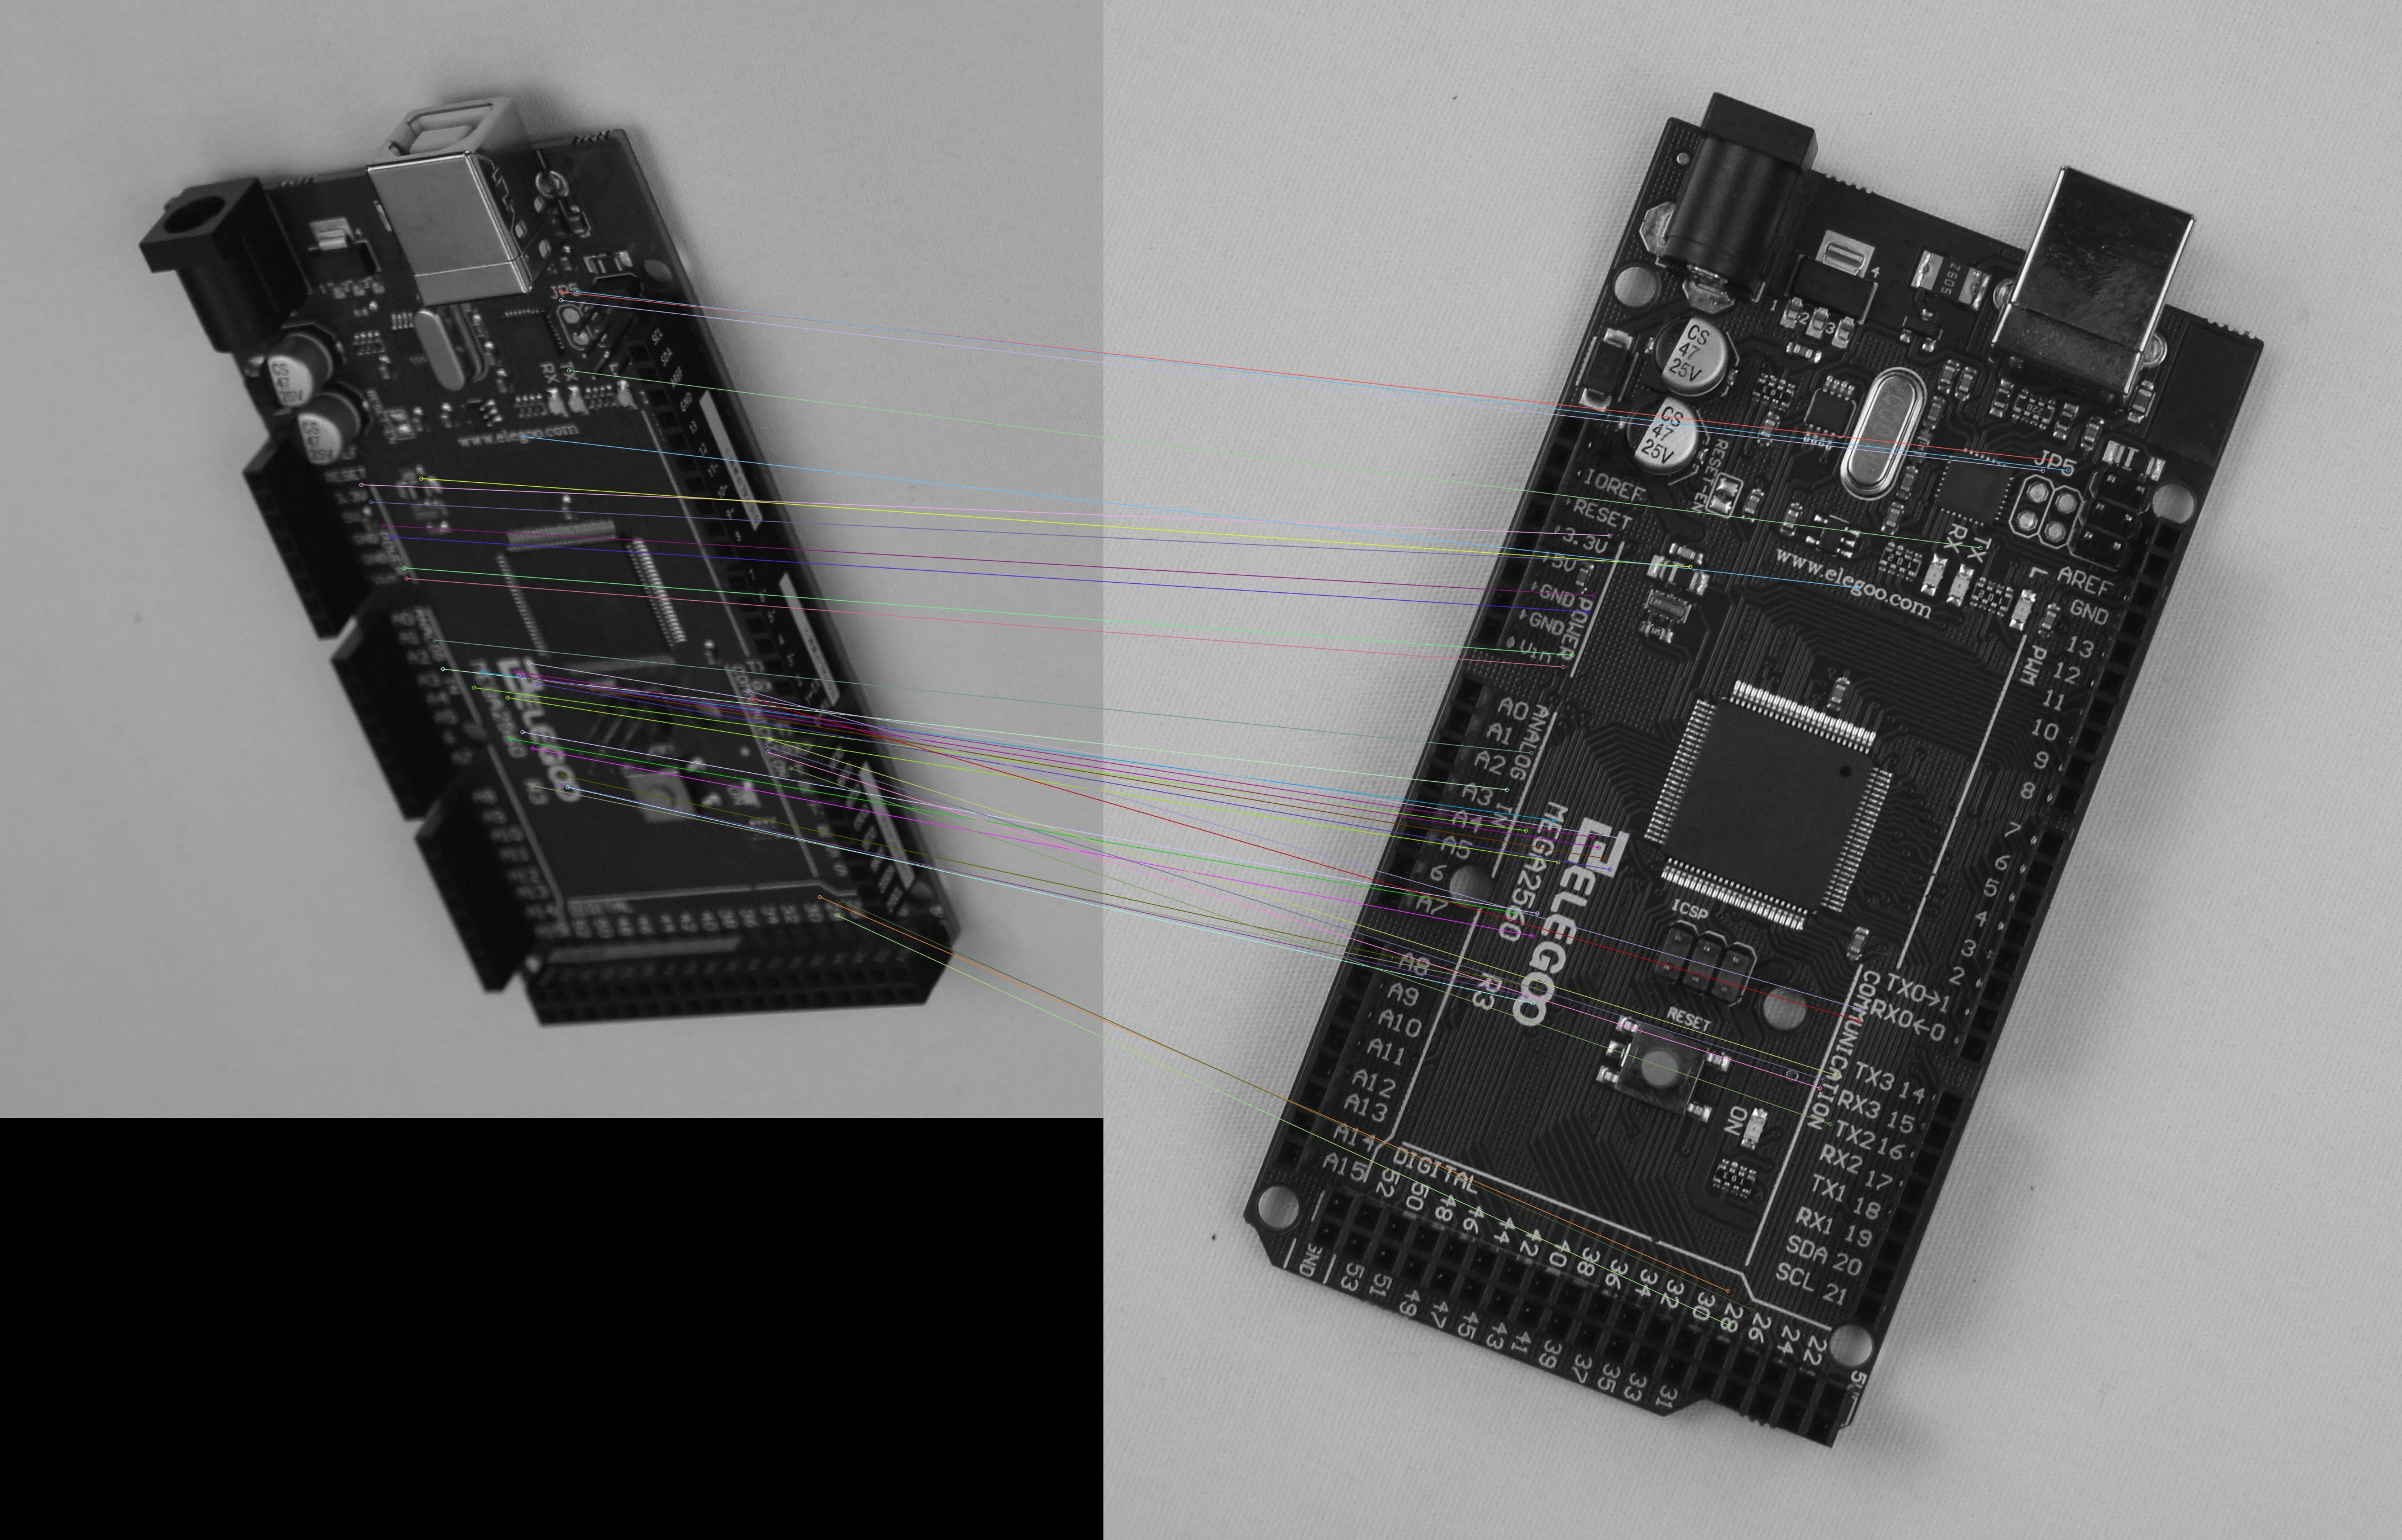
\includegraphics[width=0.9\linewidth,height=3cm]{../a02 codes/matches_AAAA1.jpg}
		\end{minipage}
		\vspace{0.15cm}
		\begin{minipage}{0.19\textwidth}
			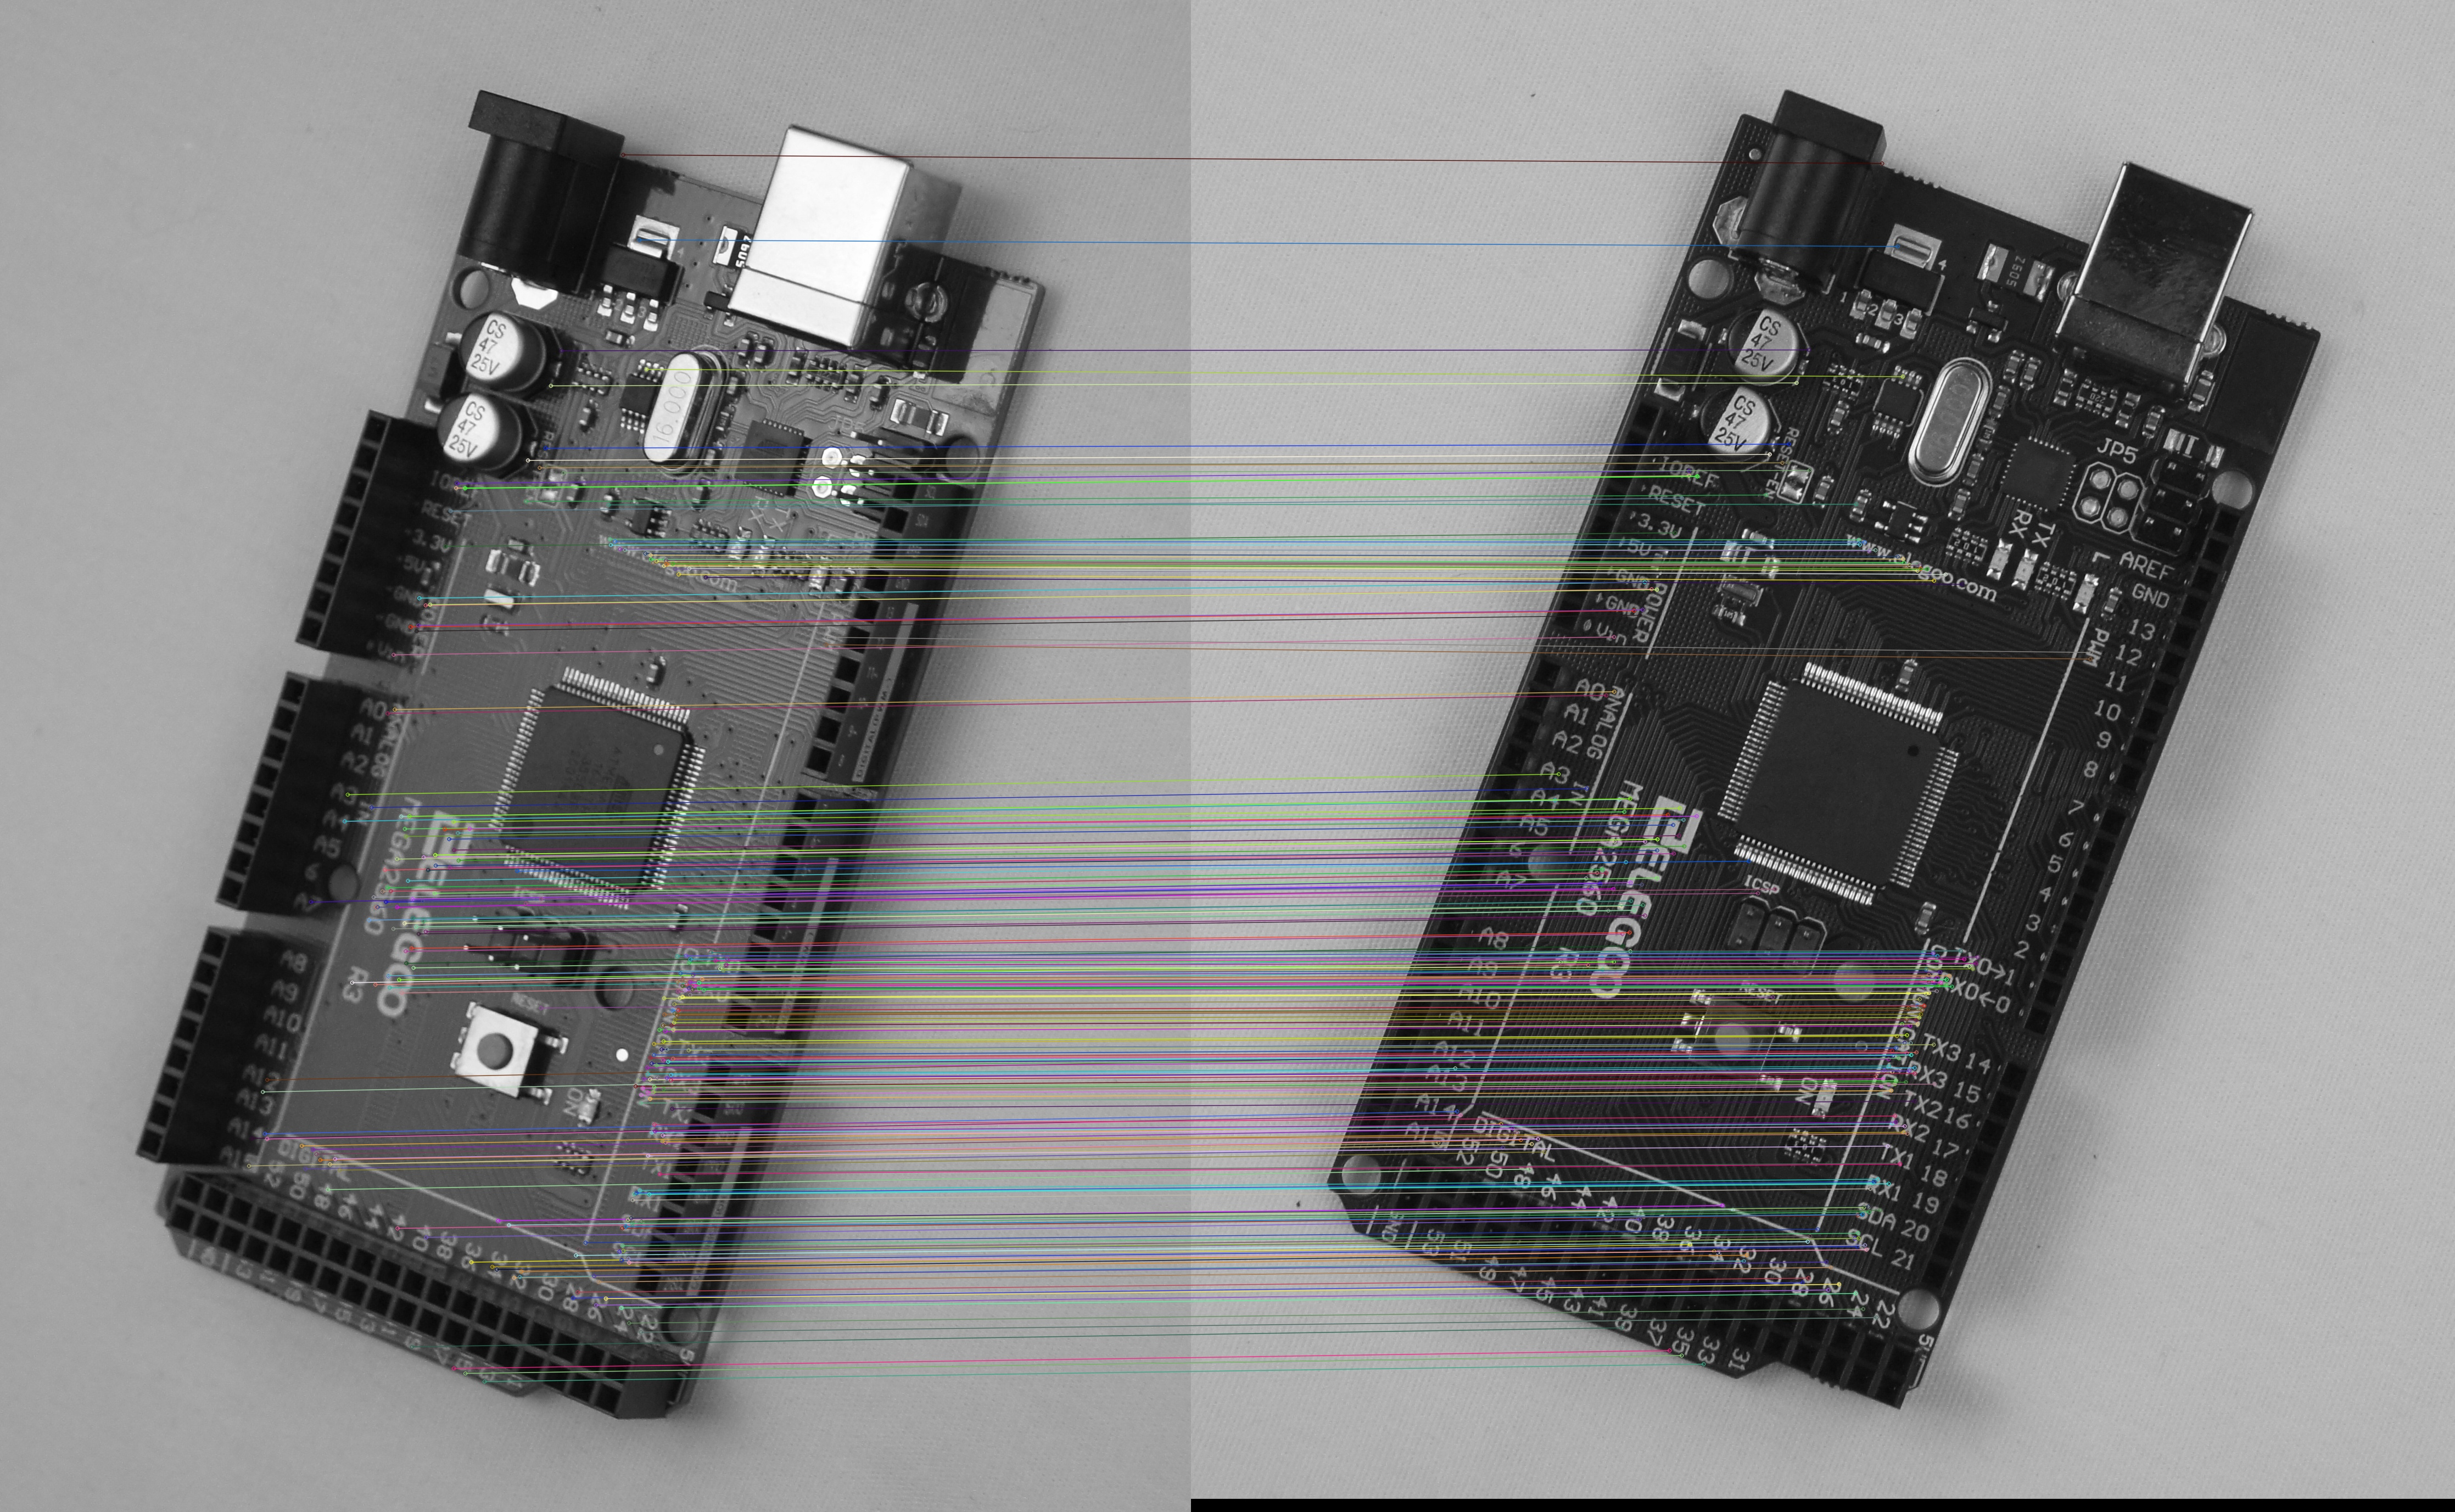
\includegraphics[width=\linewidth,height=3cm]{../a02 codes/matches_ADAD1.jpg}
		\end{minipage}\hfill
		\begin{minipage}{0.19\textwidth}
			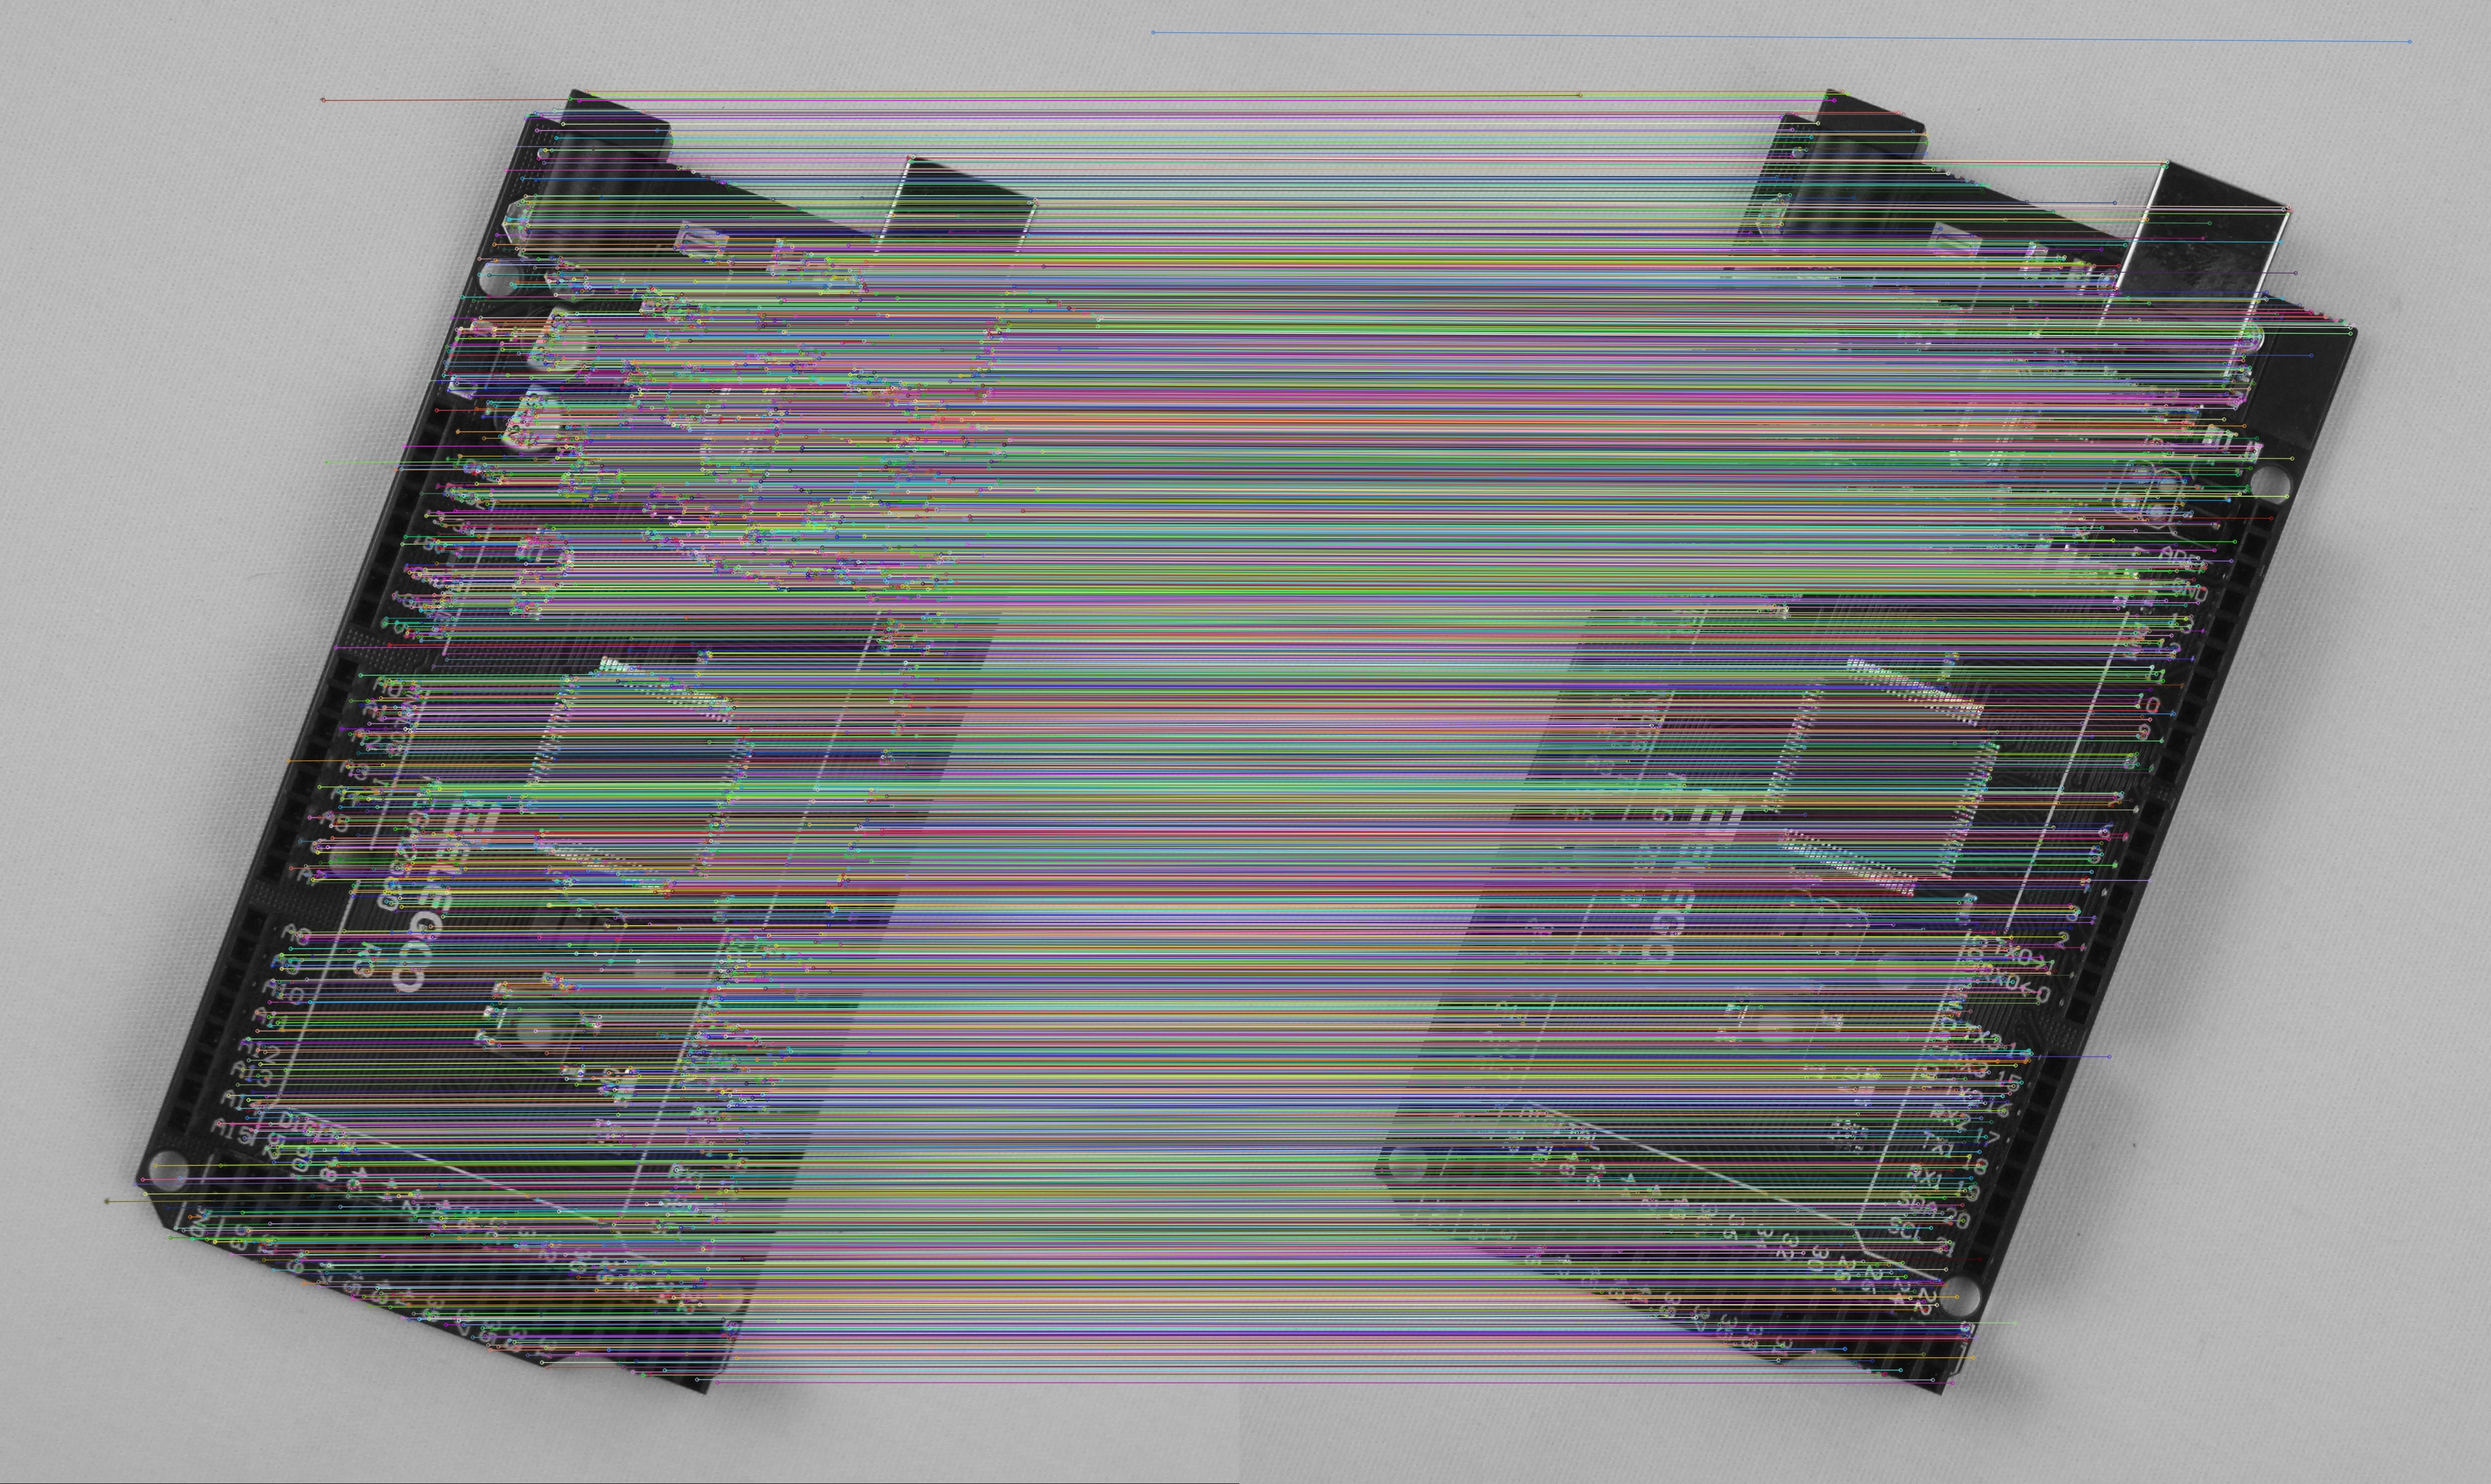
\includegraphics[width=\linewidth,height=3cm]{../a02 codes/matches_AECC2.jpg}
		\end{minipage}
		\vspace{0.15cm}
		\begin{minipage}{0.19\textwidth}
			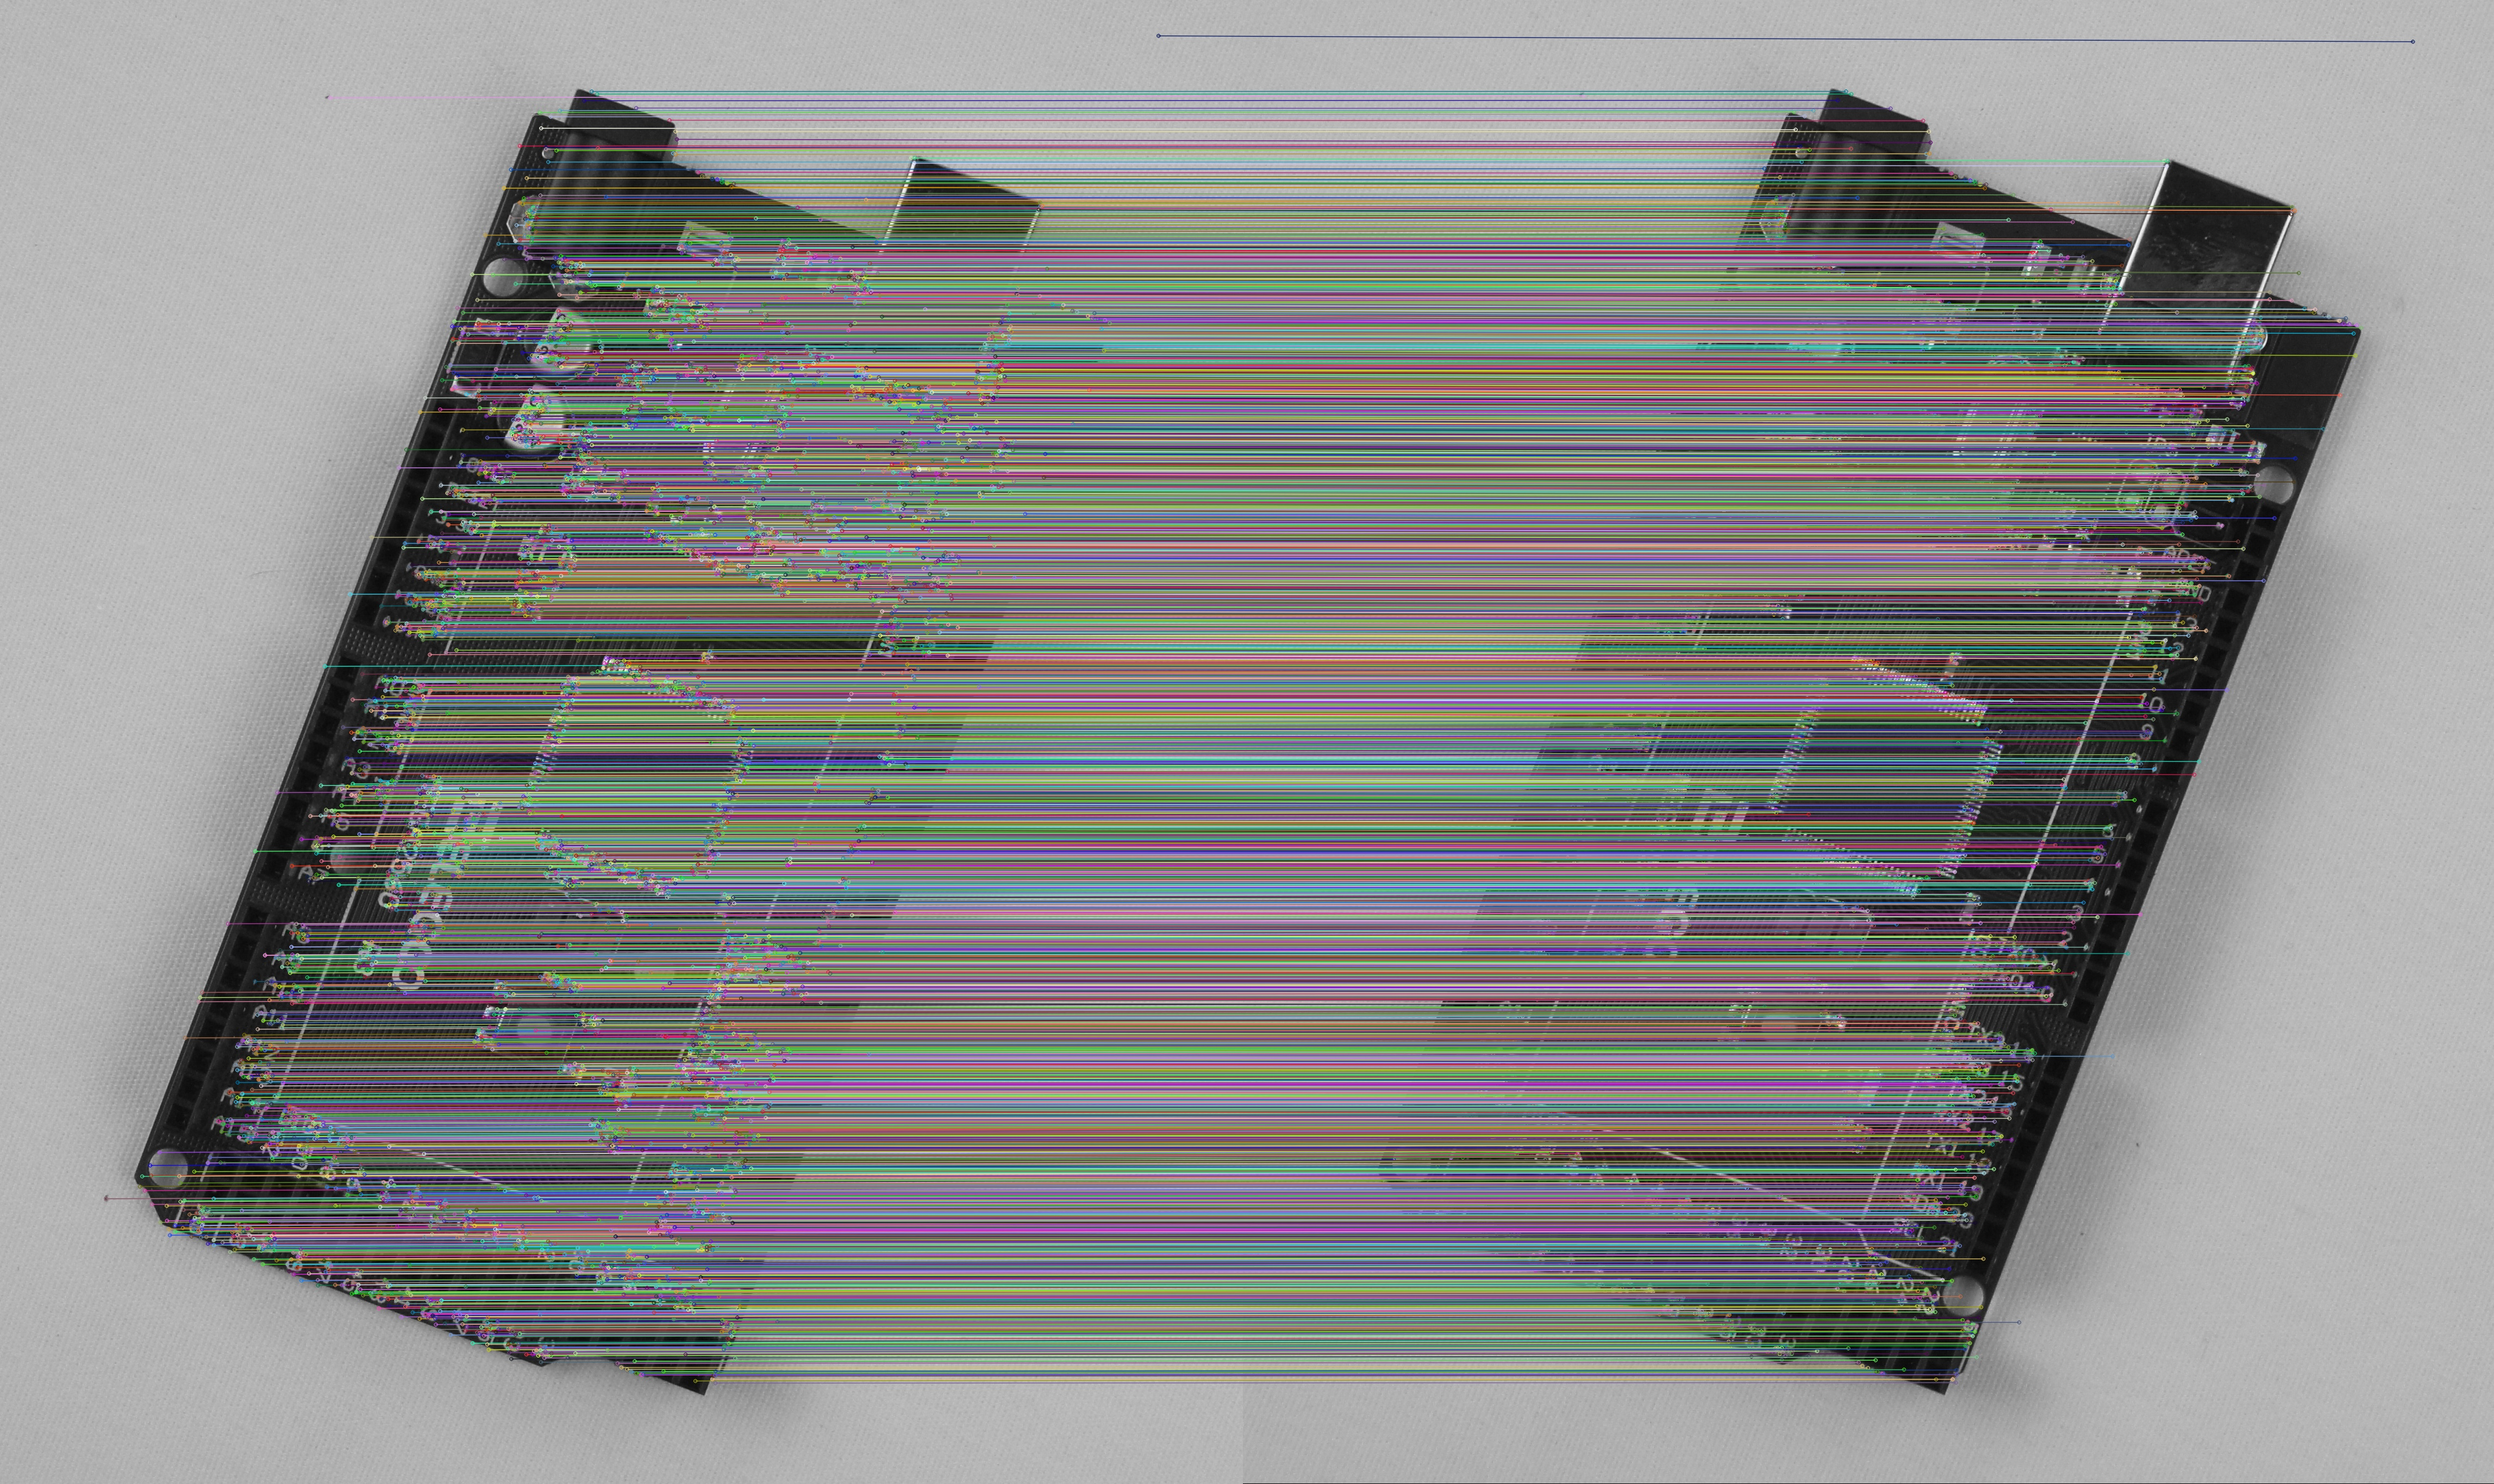
\includegraphics[width=\linewidth,height=3cm]{../a02 codes/matches_AECC3.jpg}
		\end{minipage}
		\begin{minipage}{0.19\textwidth}
			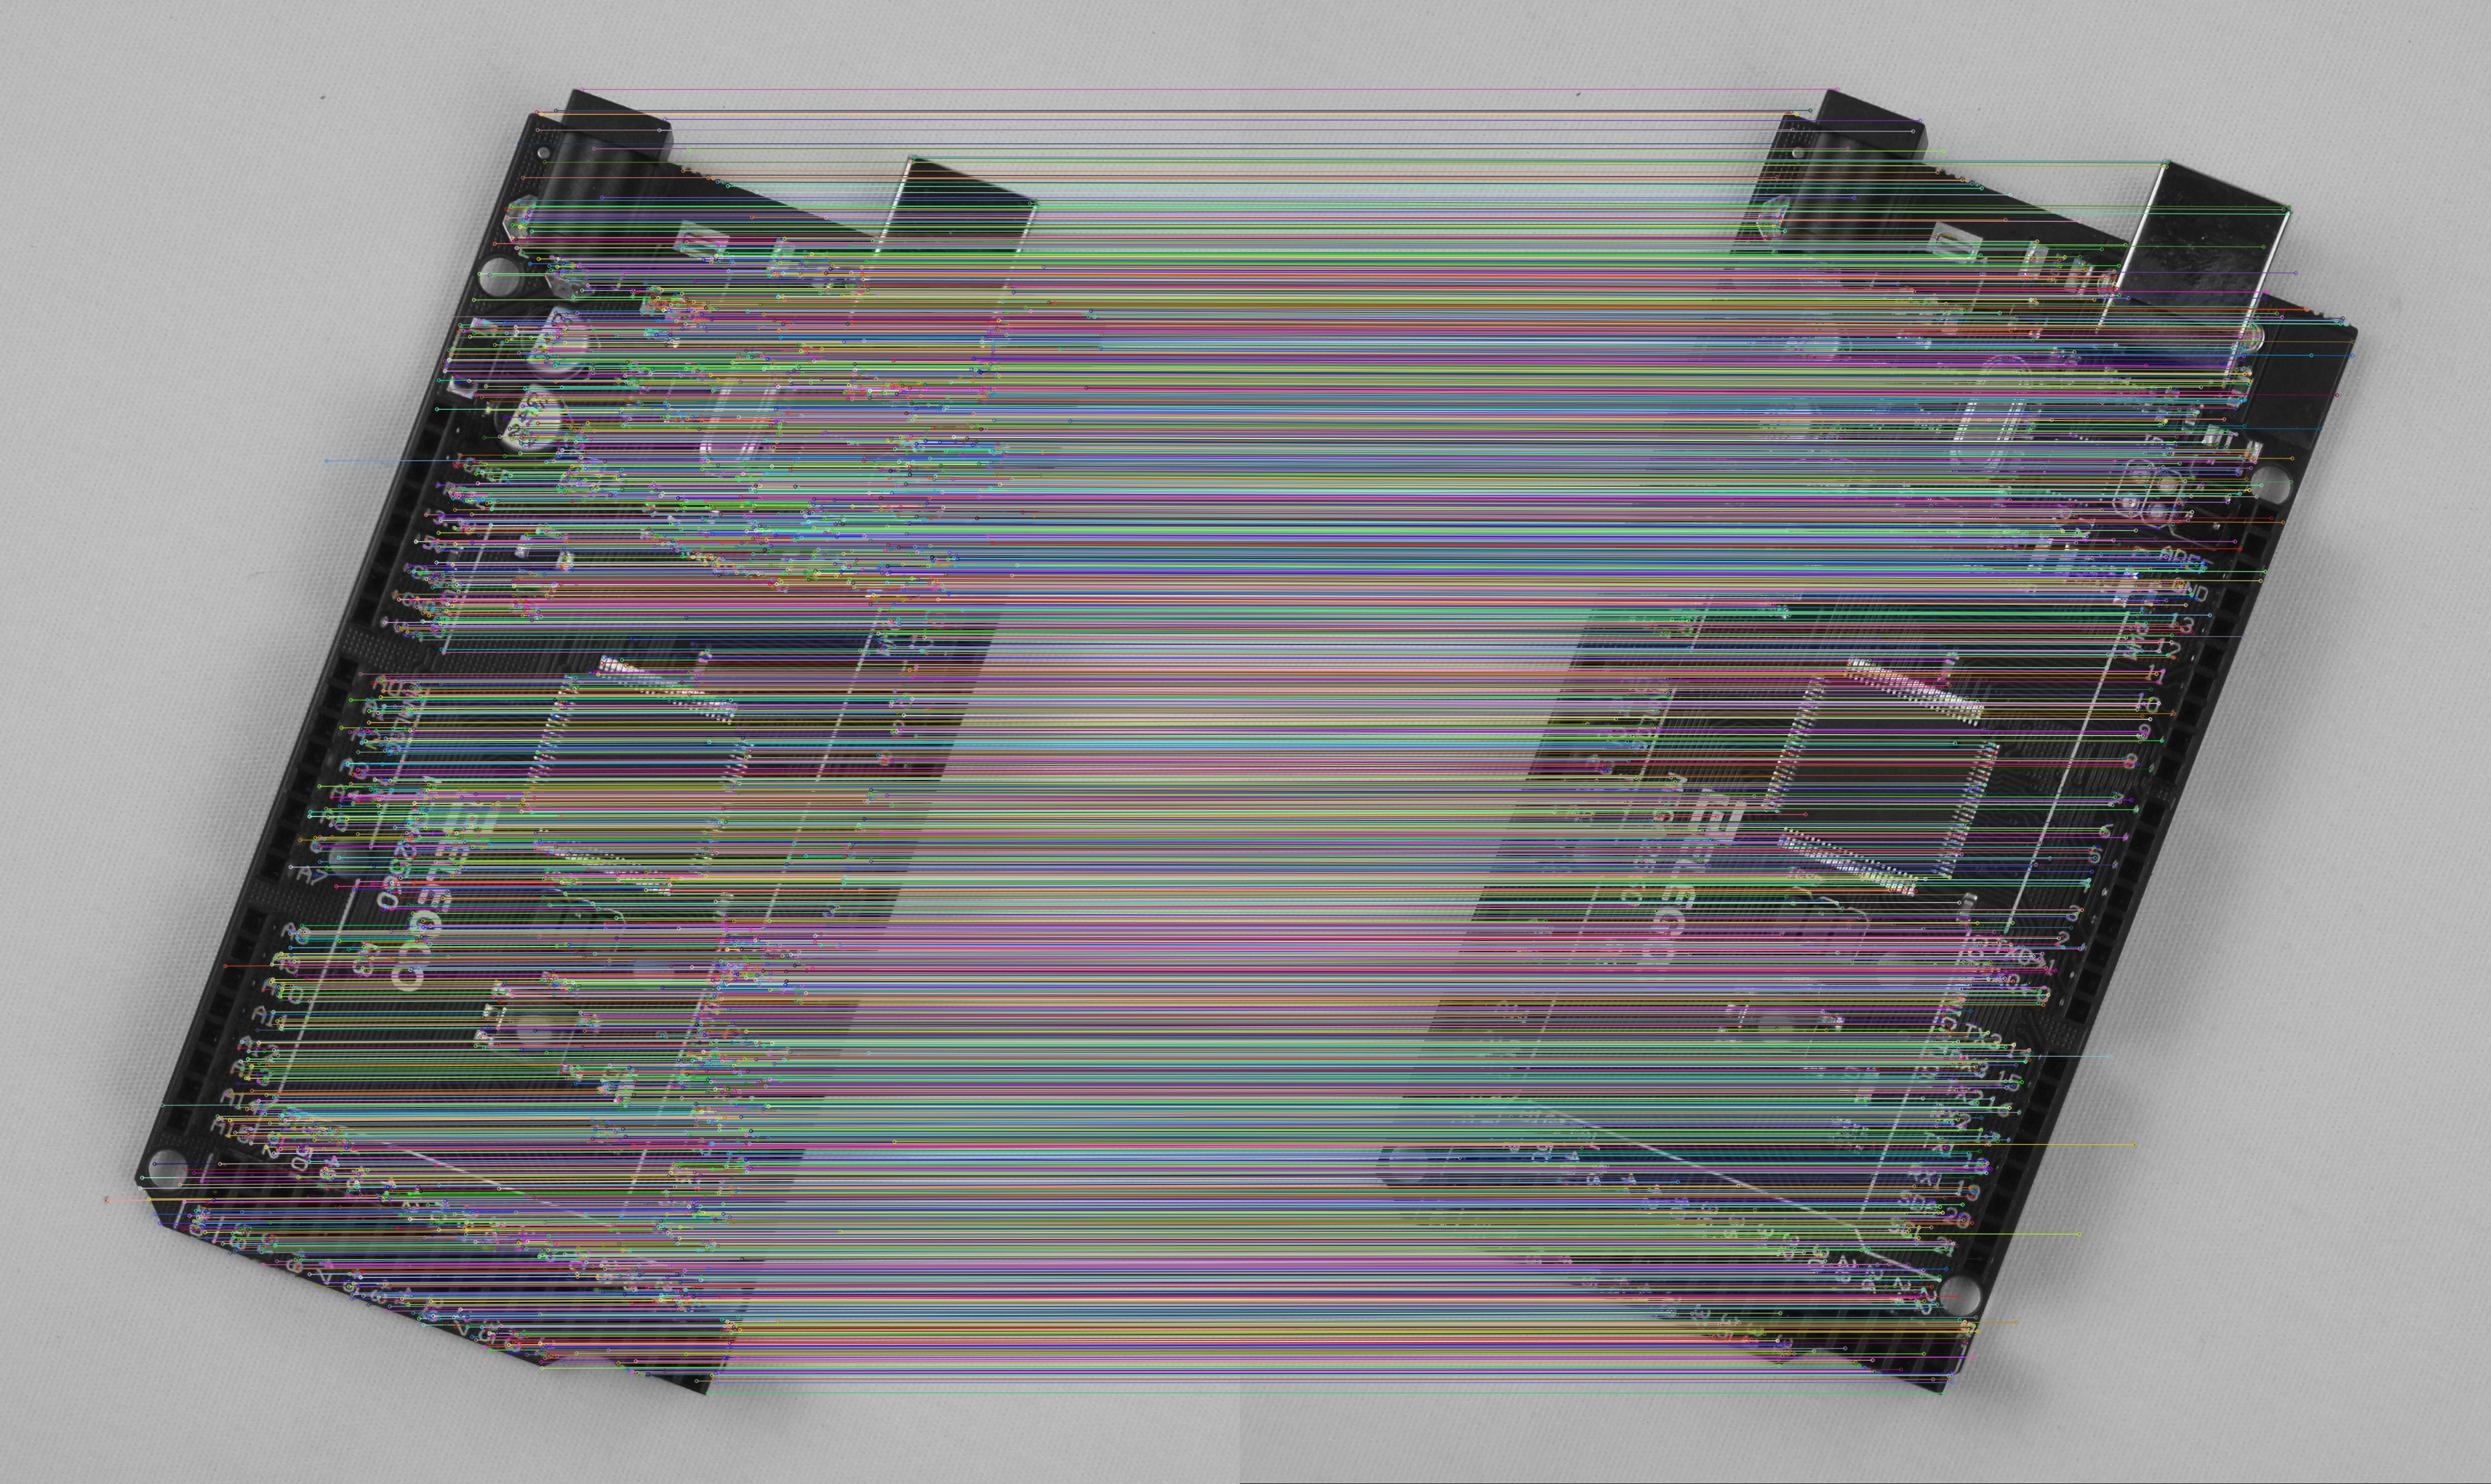
\includegraphics[width=\linewidth,height=3cm]{../a02 codes/matches_AECC4.jpg}
		\end{minipage}
		\vspace{-0.2cm}
		\caption{SIFT feature matching between all test images and the template (\texttt{AECC1.jpg}).}
	\end{figure}
	
	\begin{figure}[h!]
		\centering
		% Adjust the names to match your test image files
		\begin{minipage}{0.19\textwidth}
			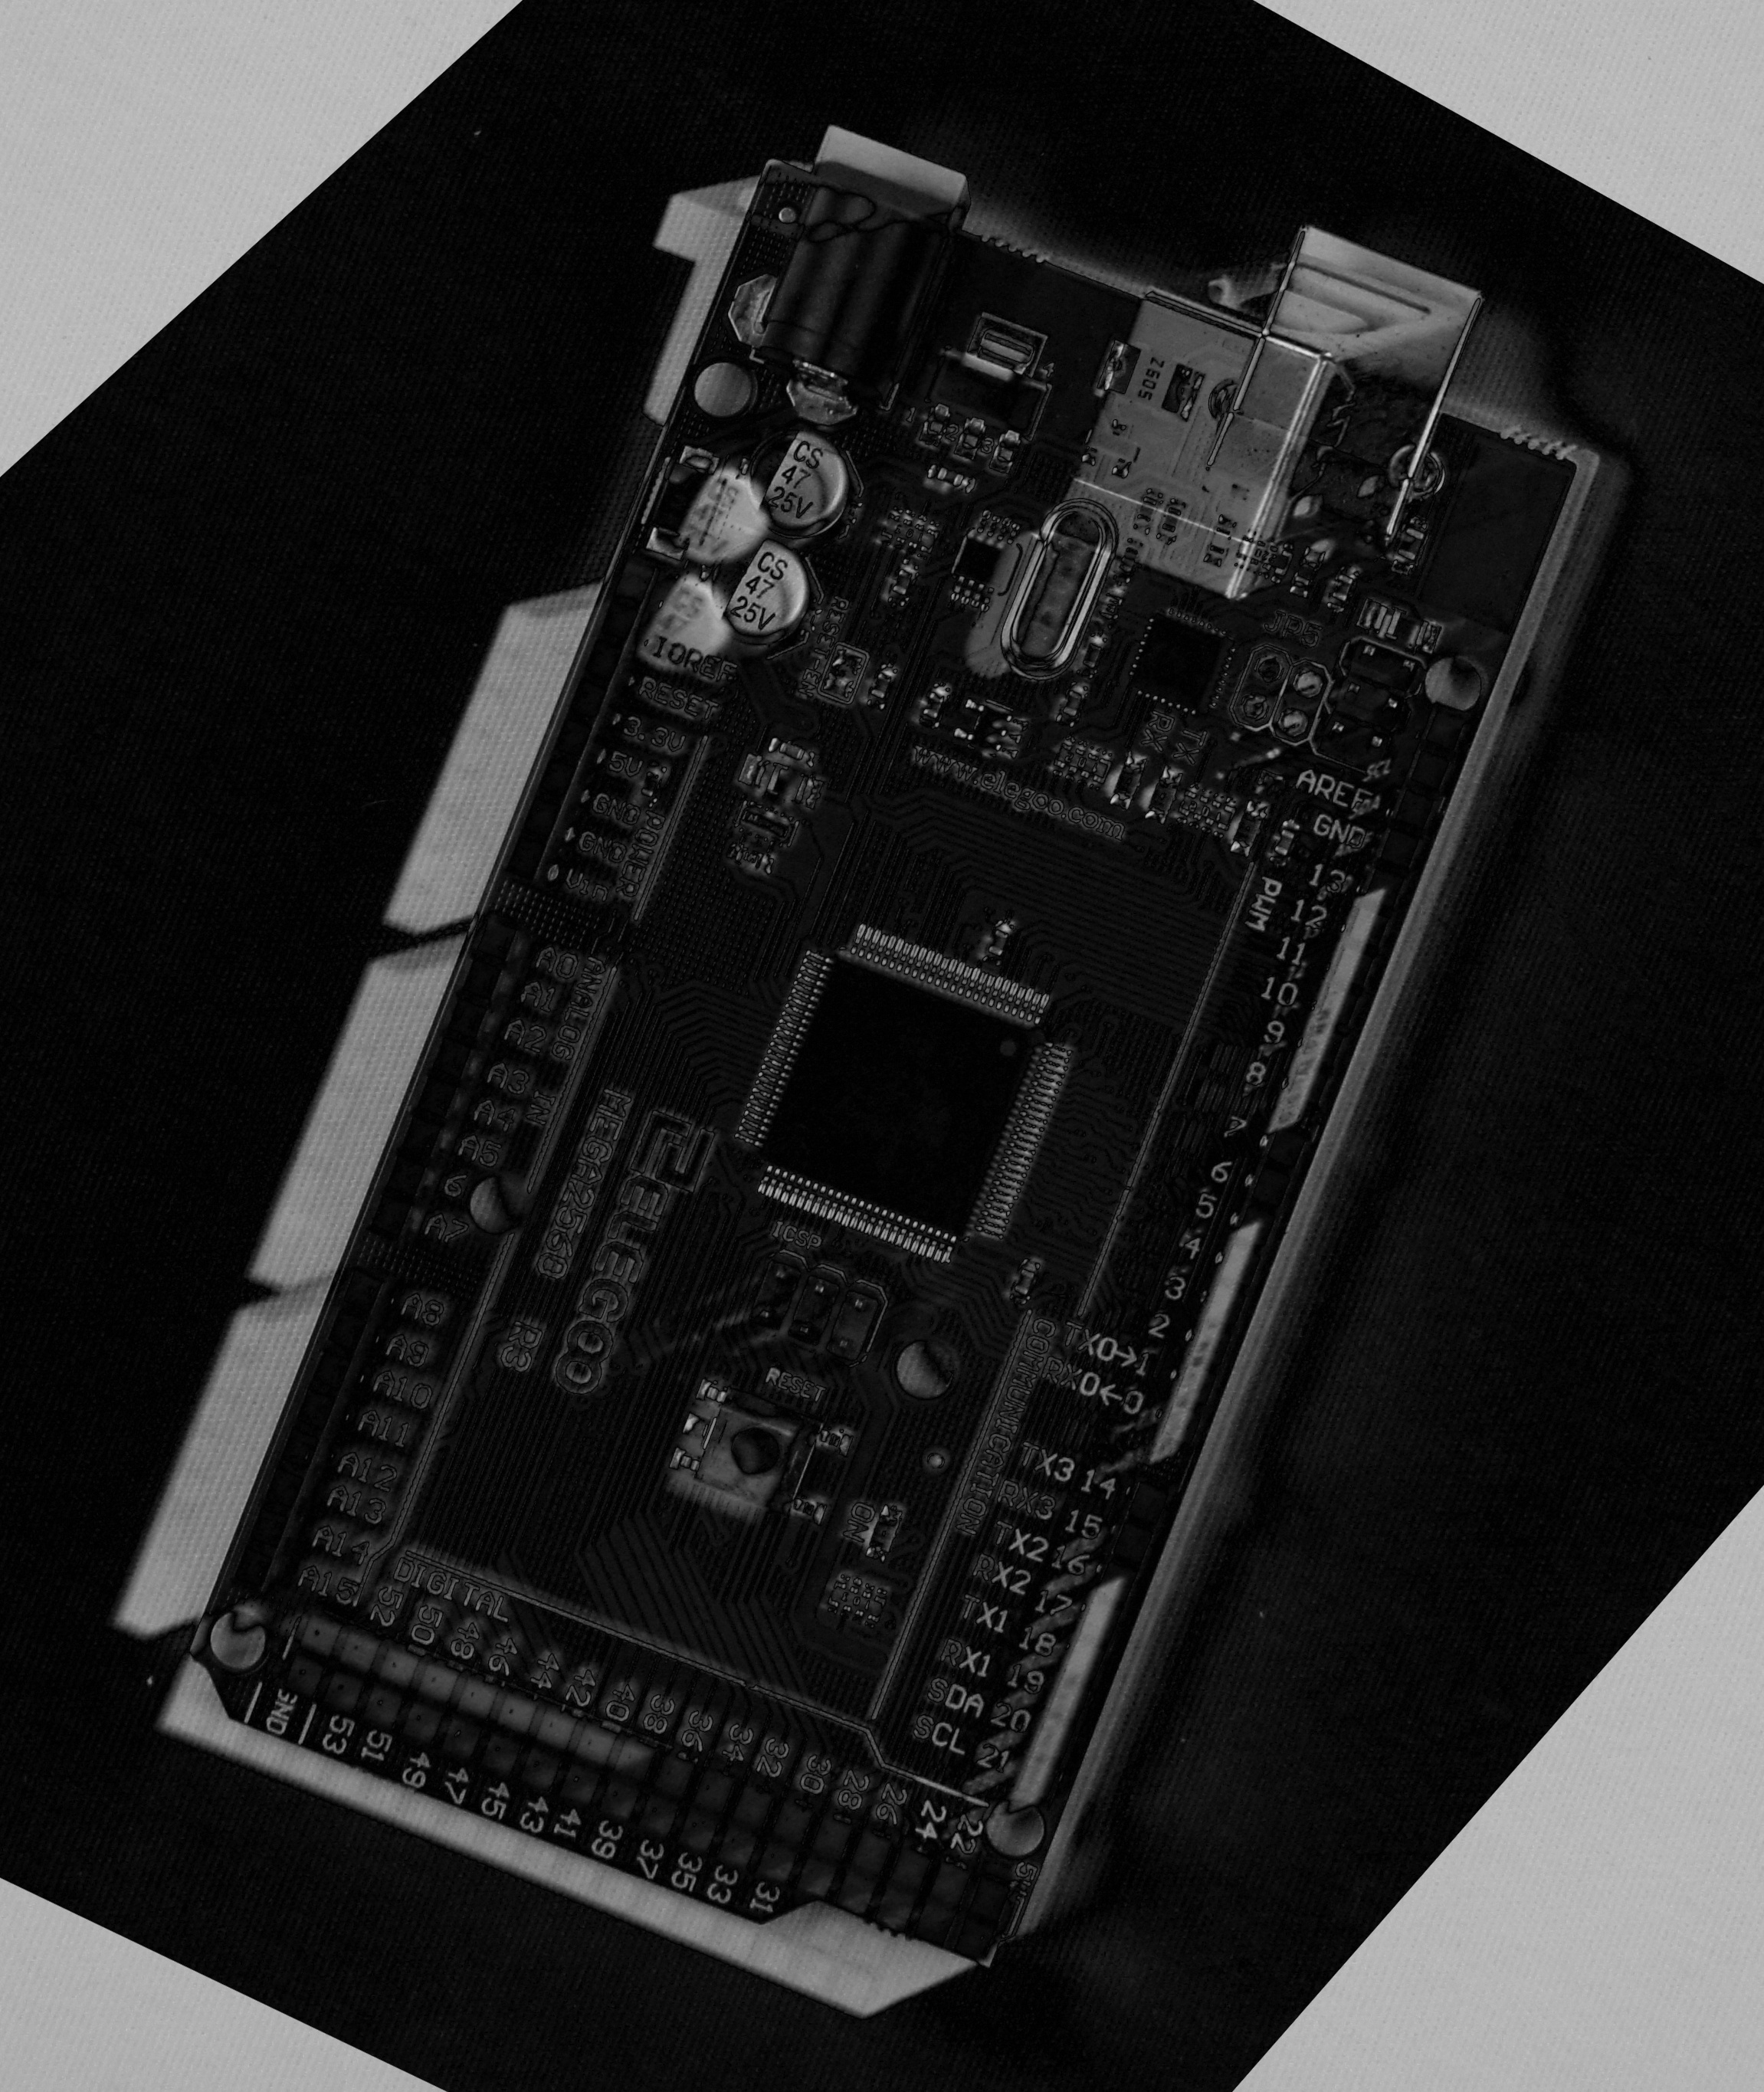
\includegraphics[width=\linewidth]{../a02 codes/diff_AAAA1.jpg}
		\end{minipage}\hfill
		\begin{minipage}{0.19\textwidth}
			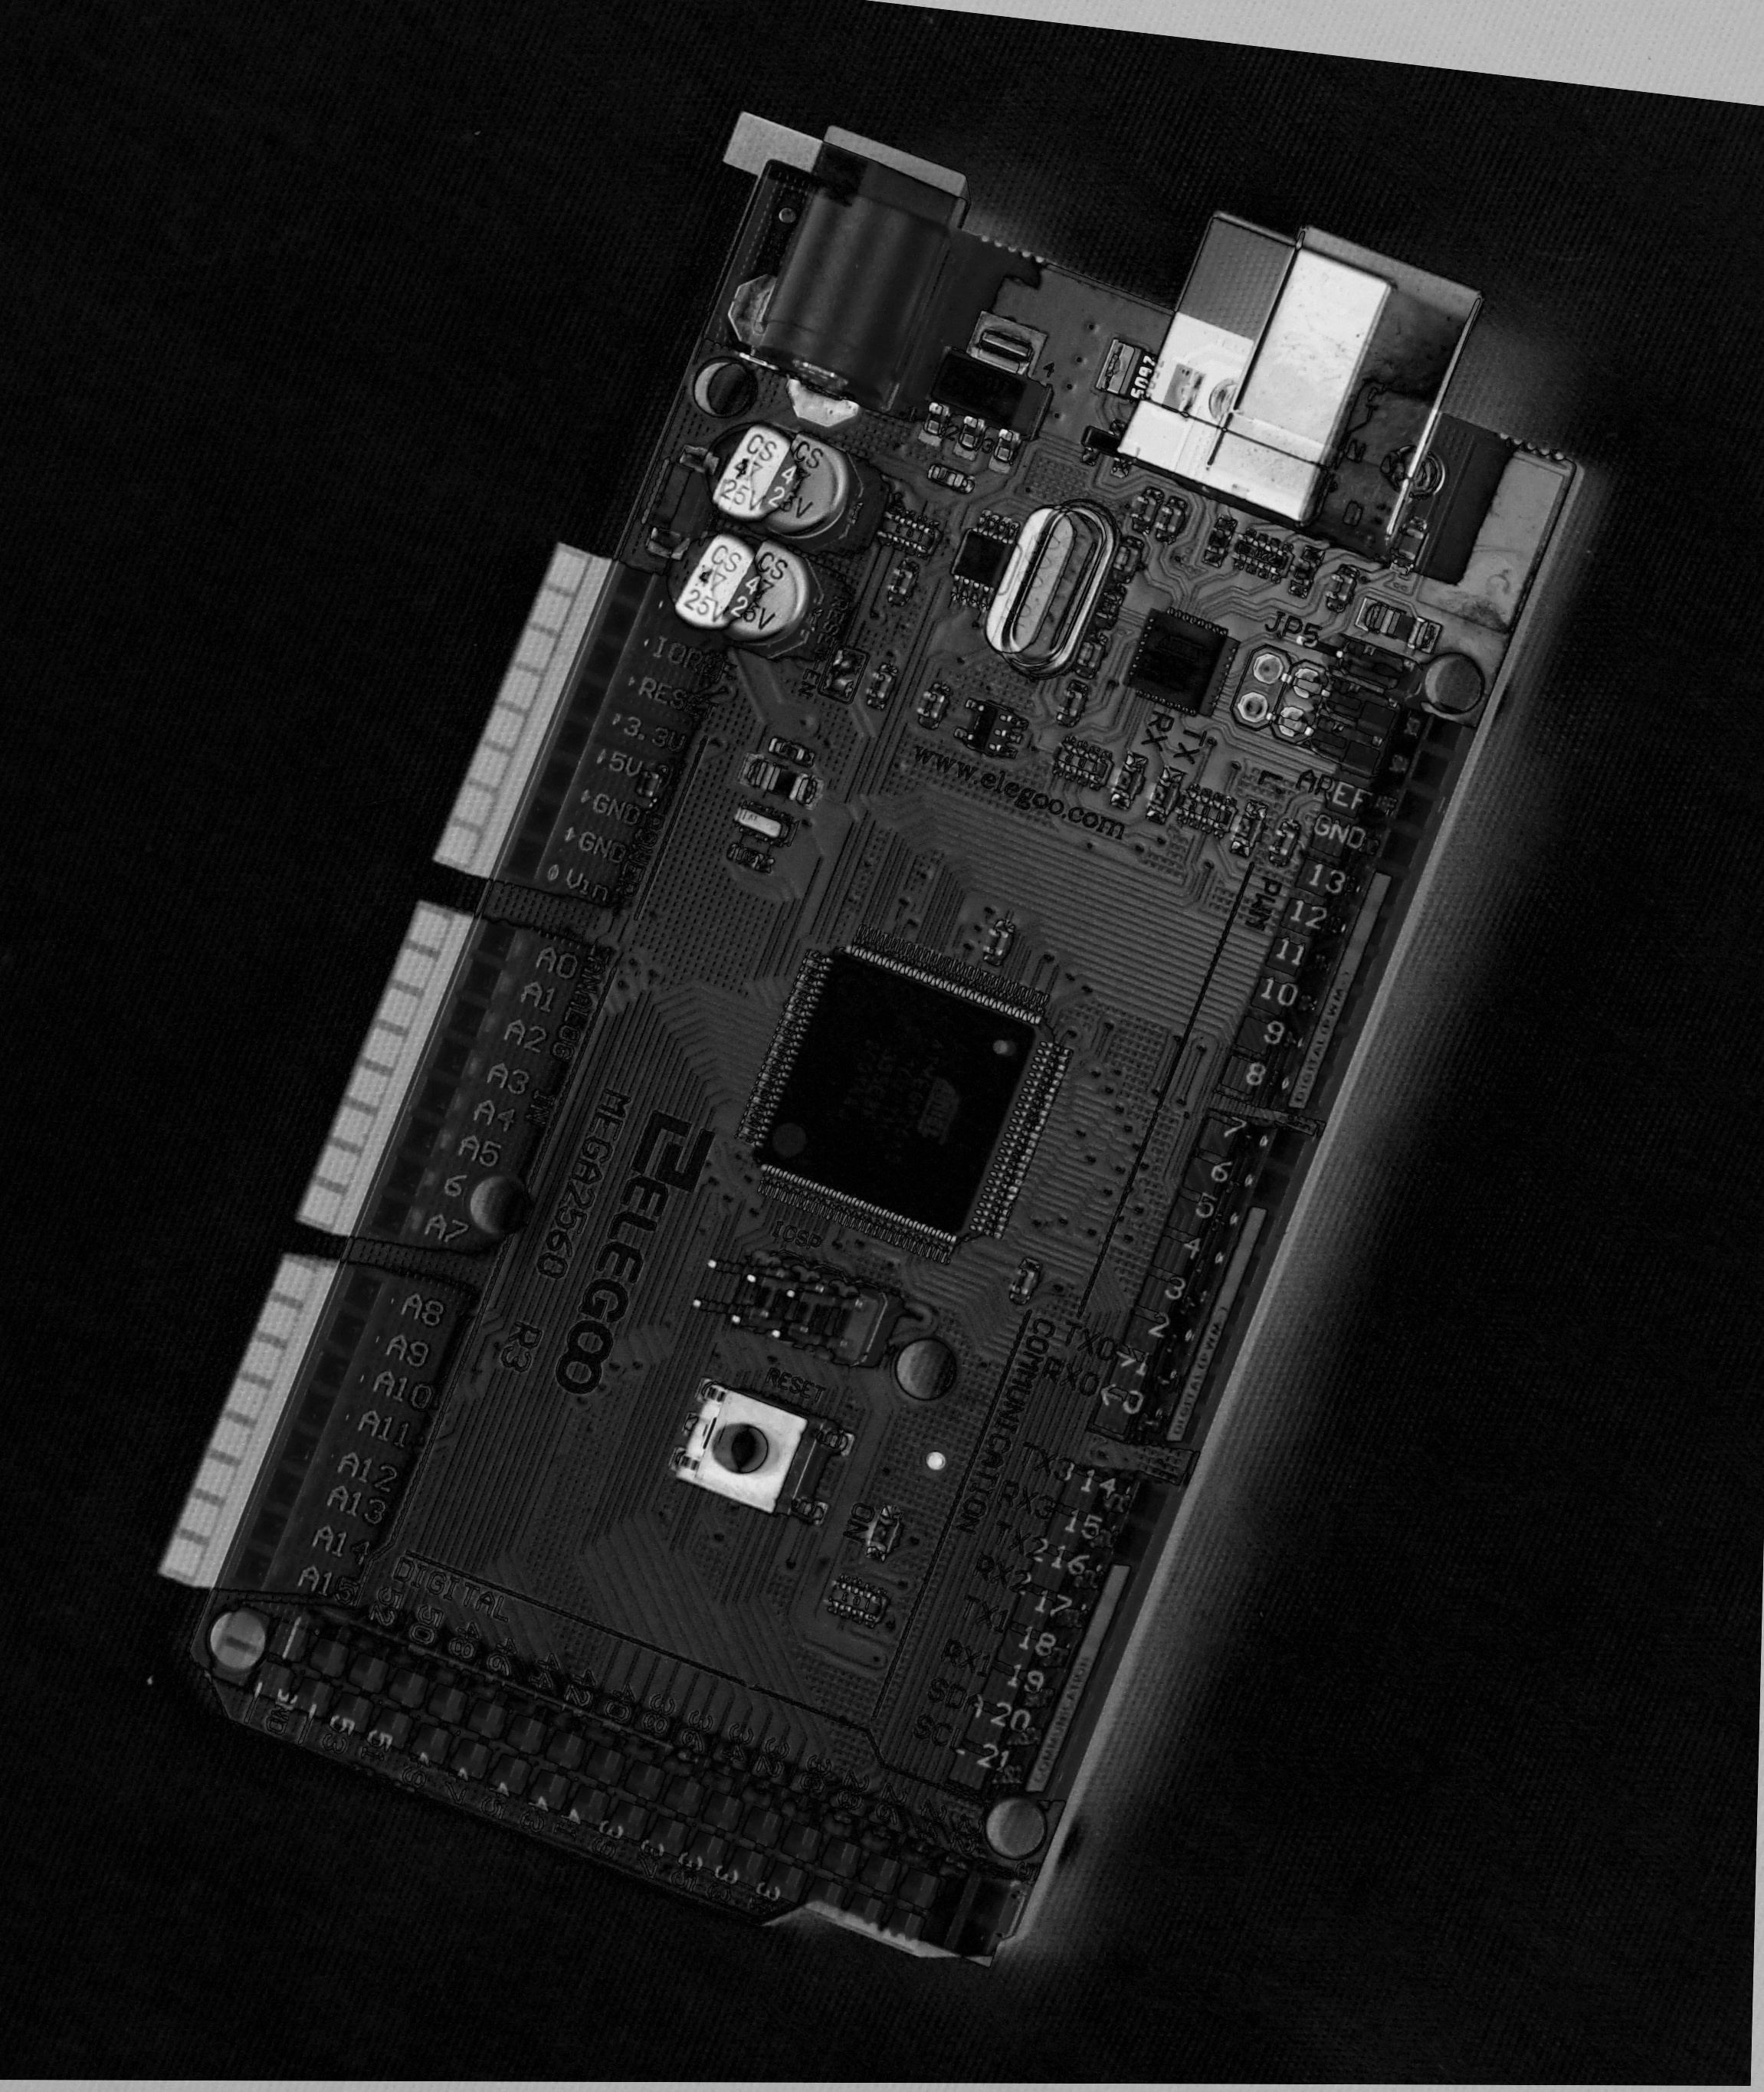
\includegraphics[width=\linewidth]{../a02 codes/diff_ADAD1.jpg}
		\end{minipage}\hfill
		\begin{minipage}{0.19\textwidth}
			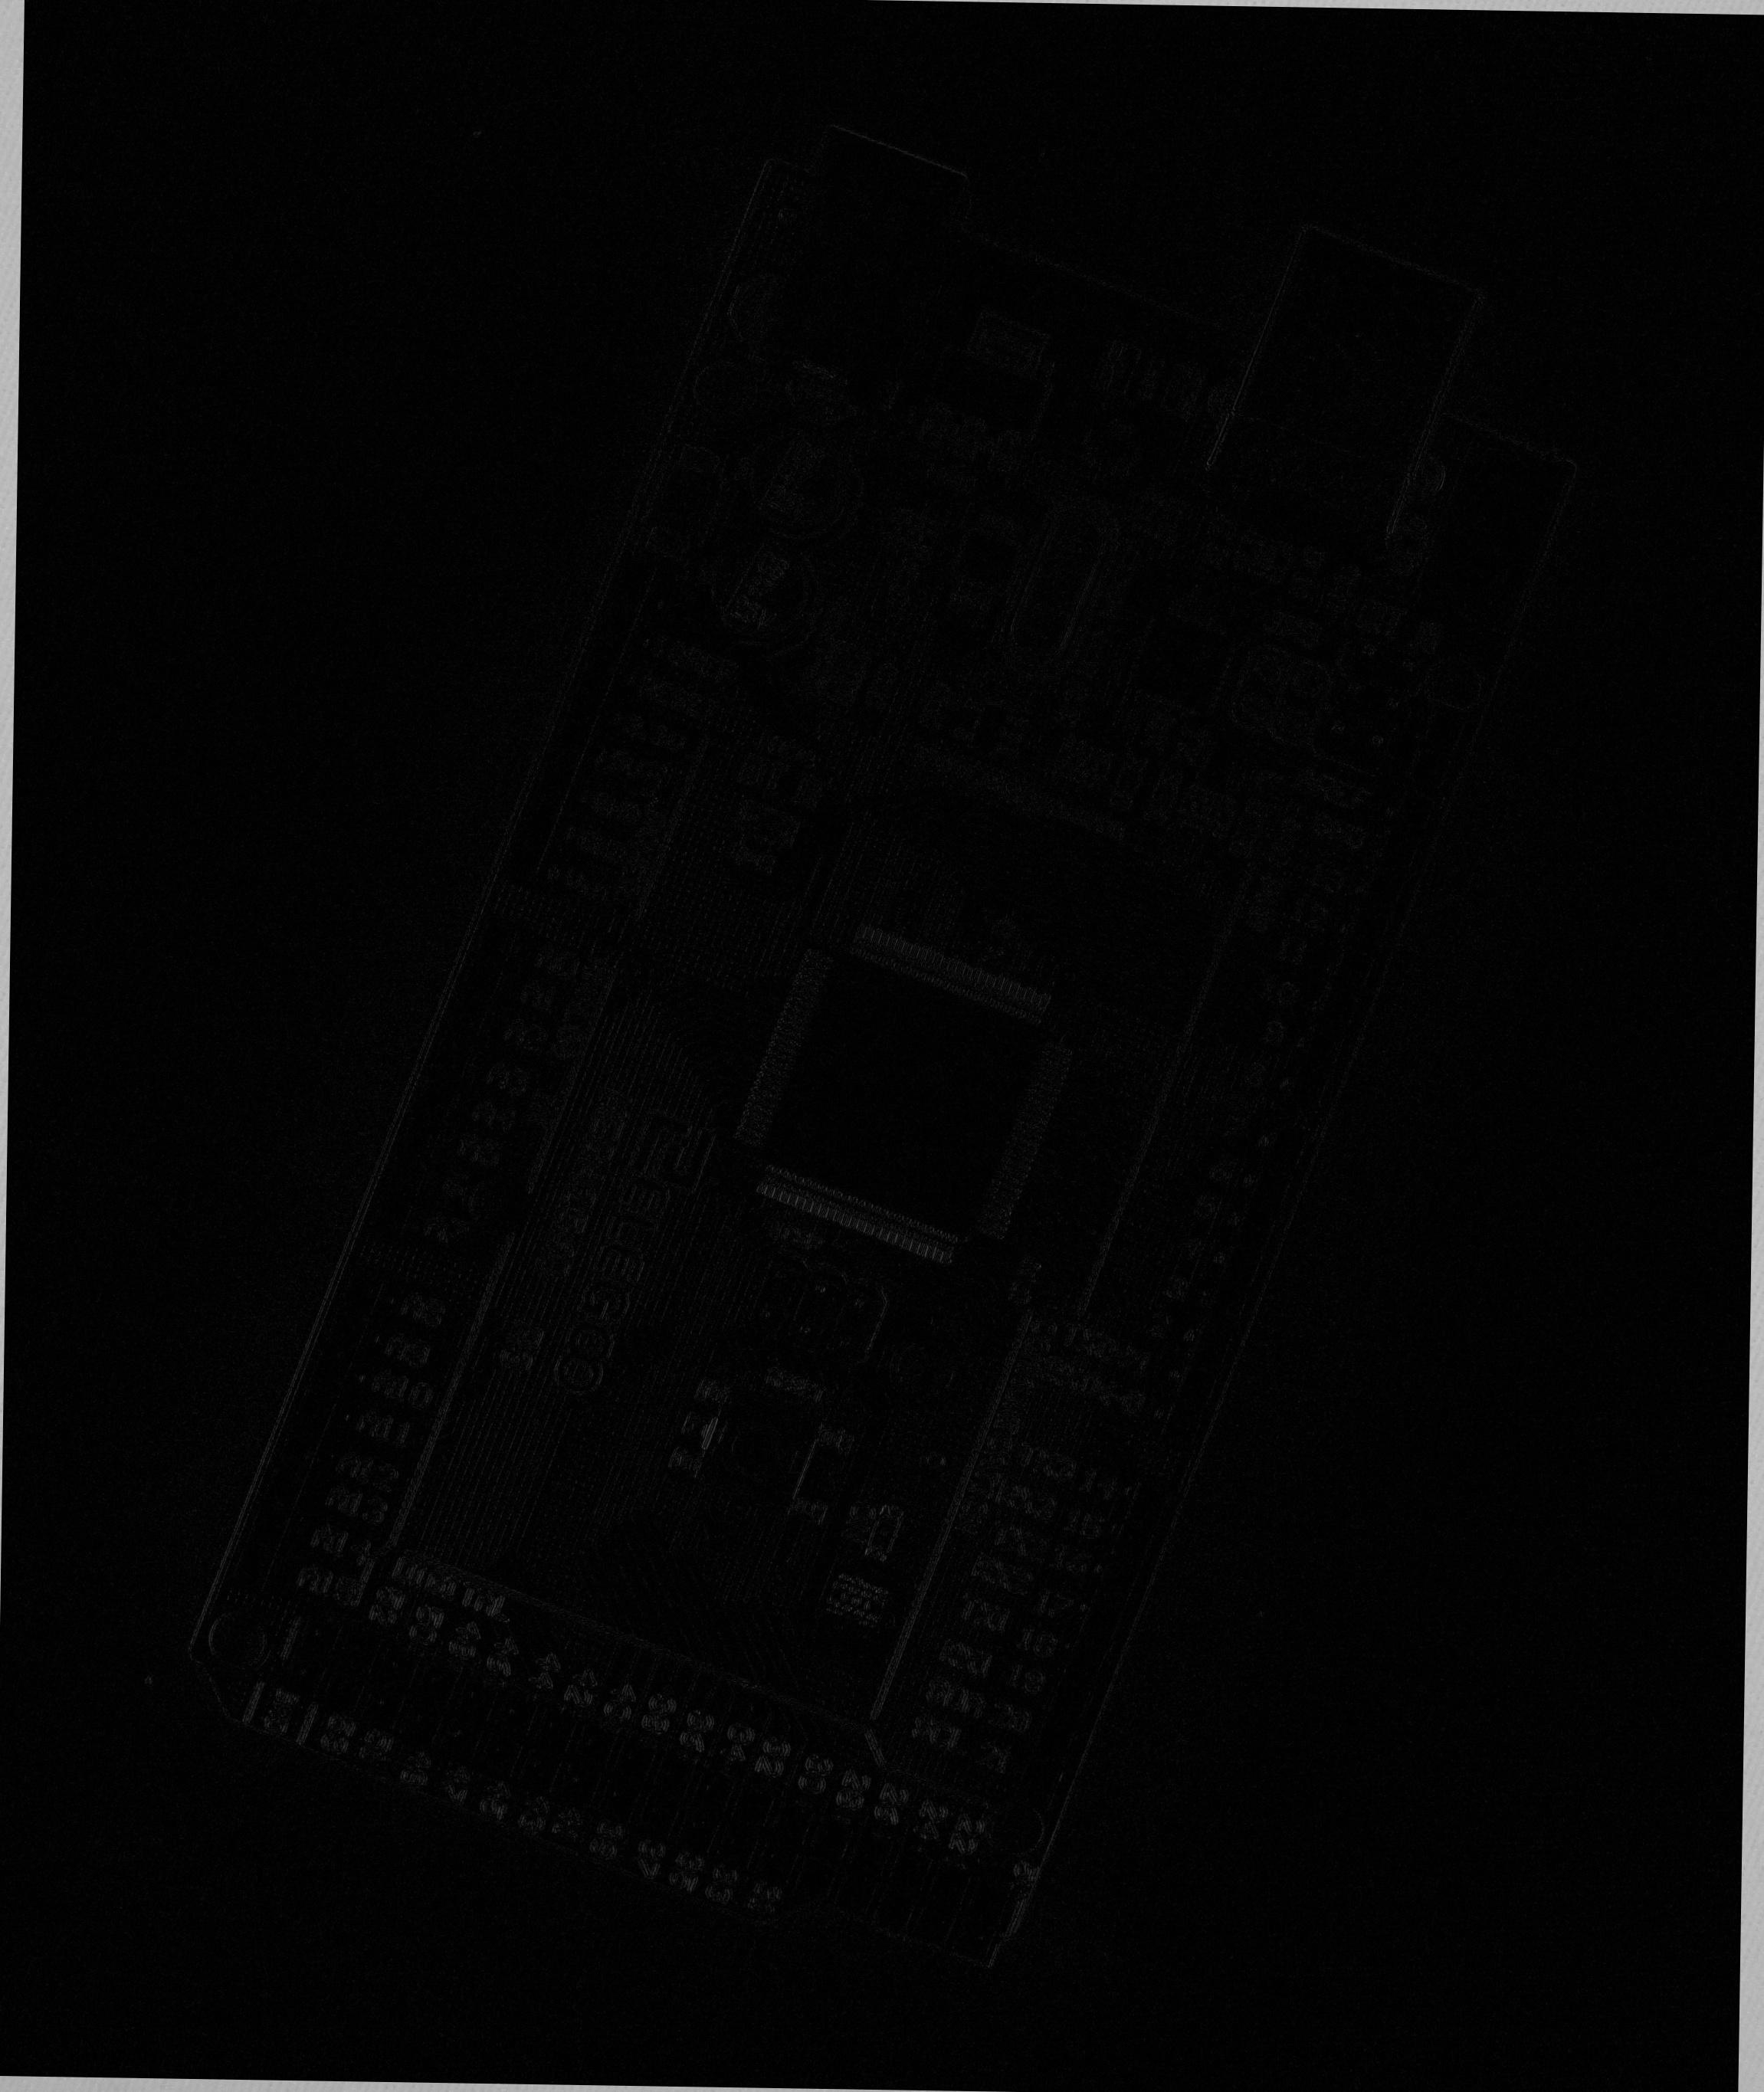
\includegraphics[width=\linewidth]{../a02 codes/diff_AECC2.jpg}
		\end{minipage}\hfill
		\begin{minipage}{0.19\textwidth}
			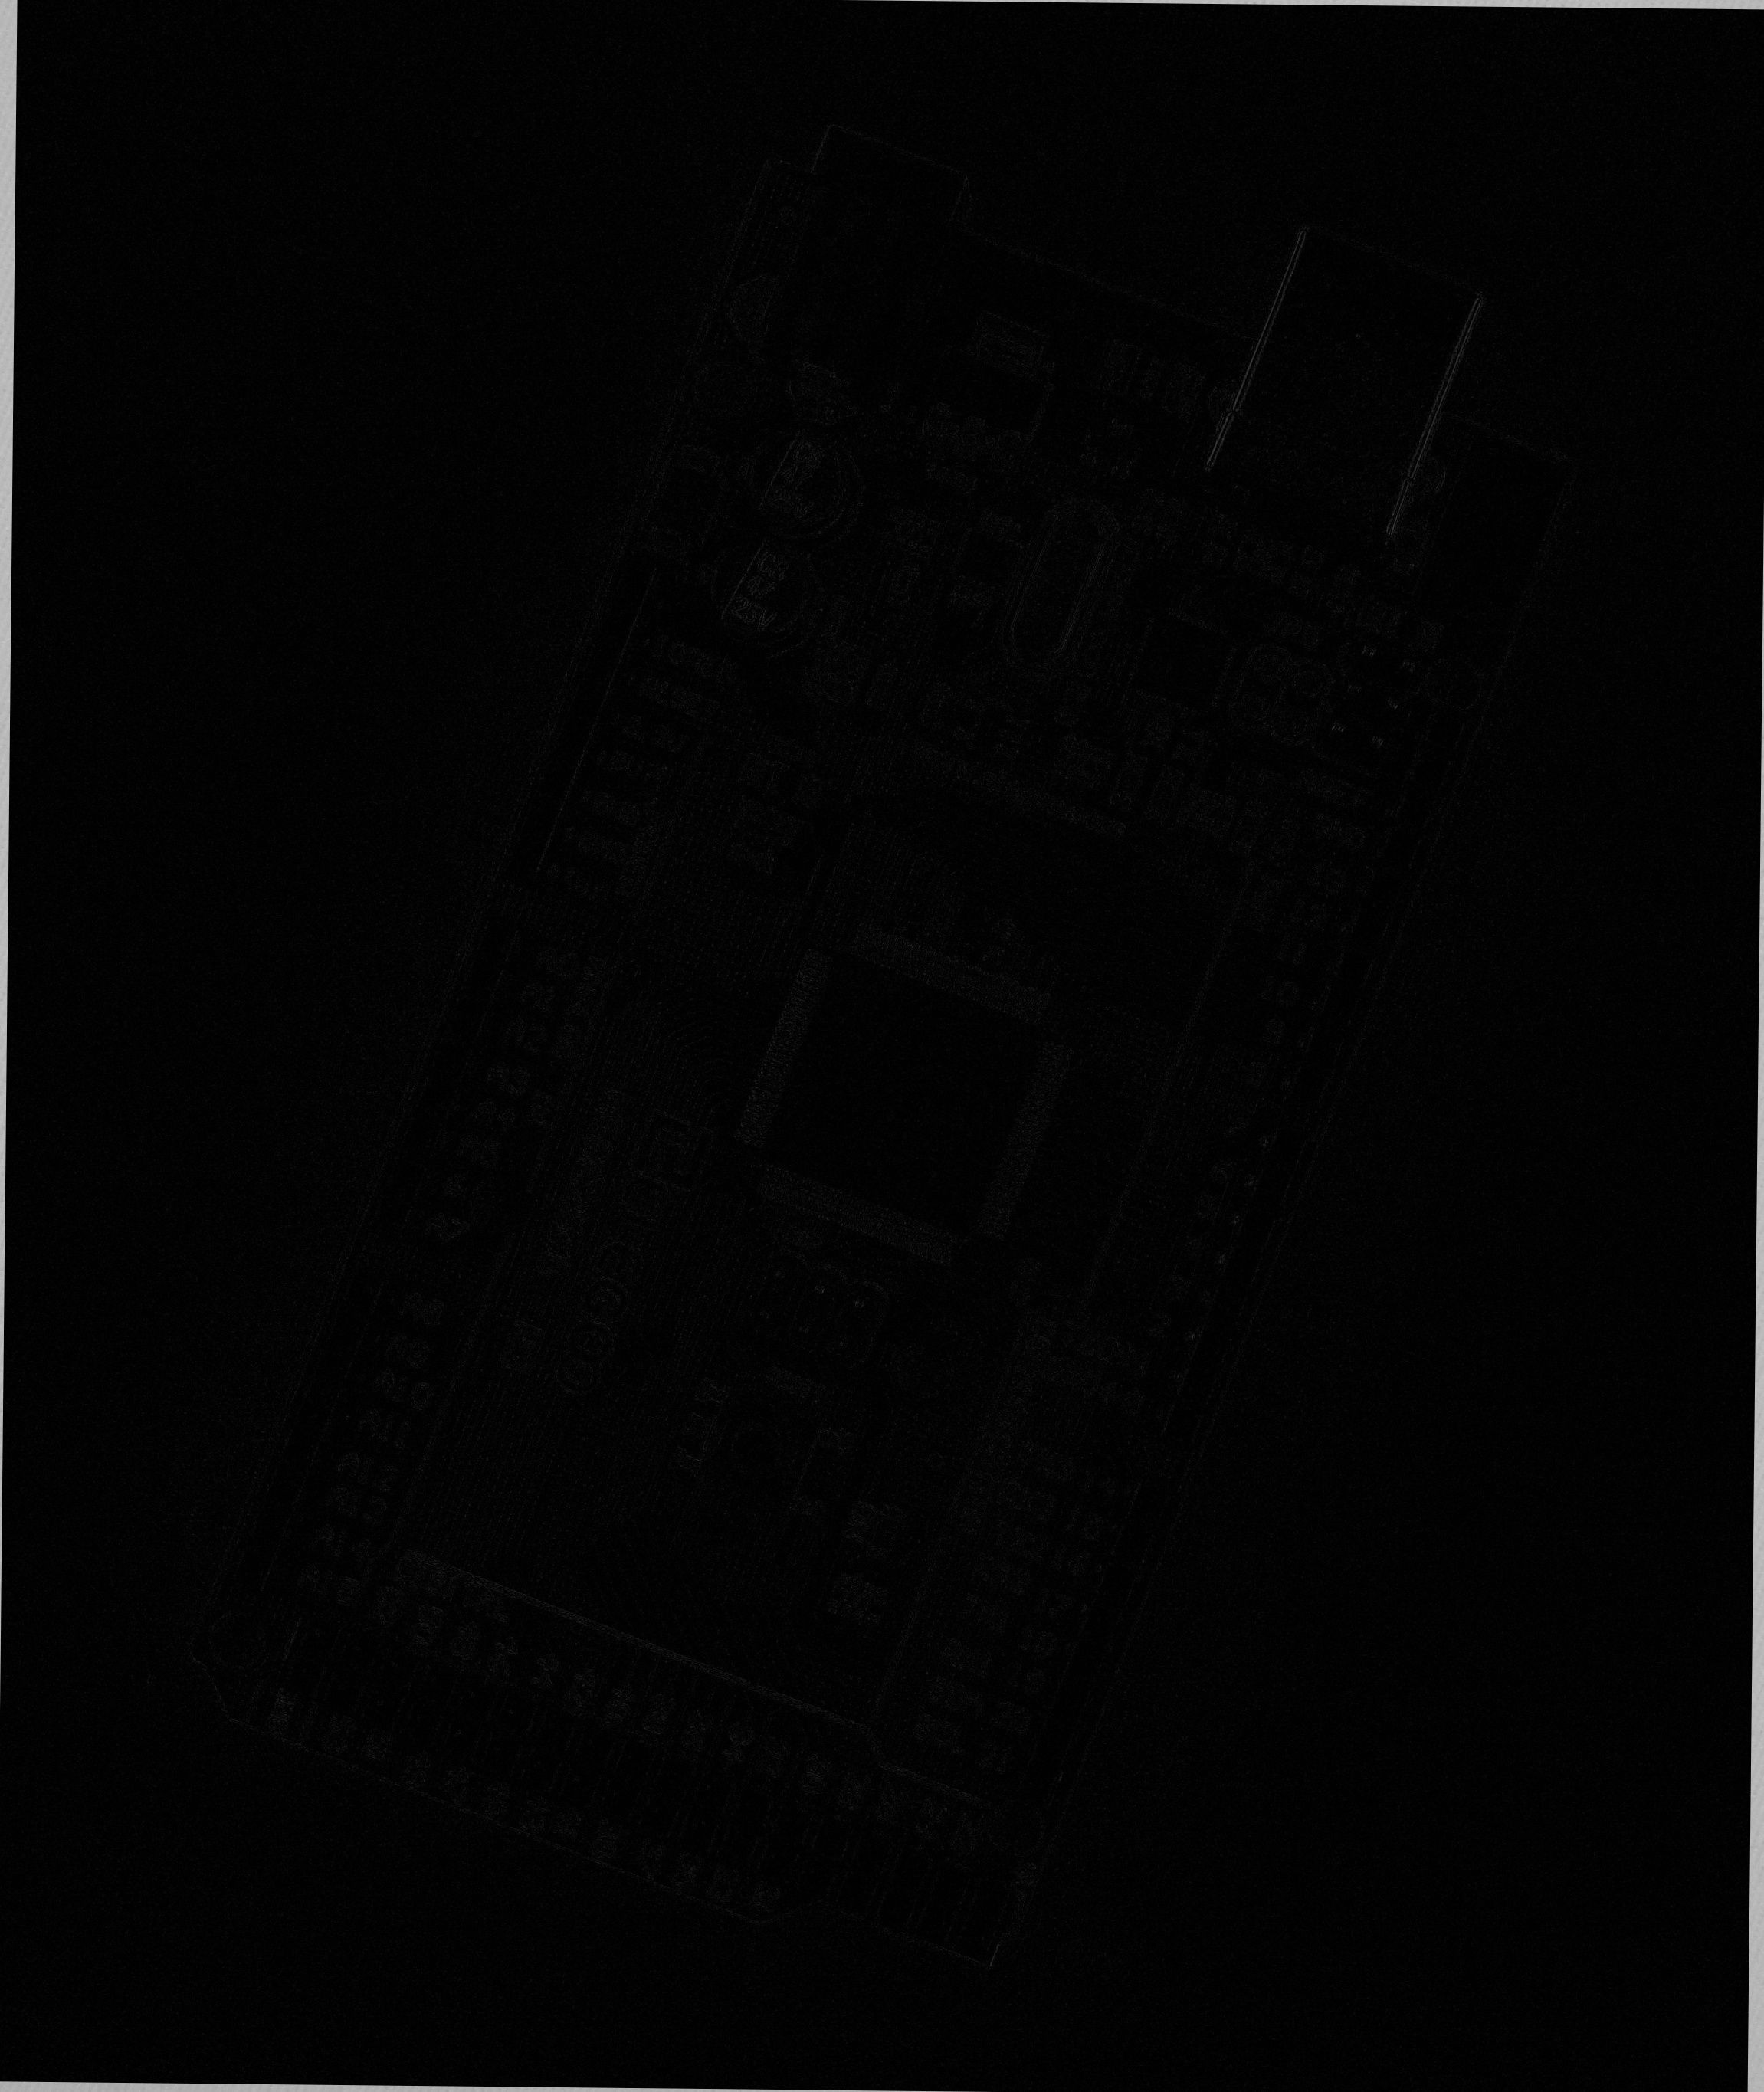
\includegraphics[width=\linewidth]{../a02 codes/diff_AECC3.jpg}
		\end{minipage}\hfill
		\begin{minipage}{0.19\textwidth}
			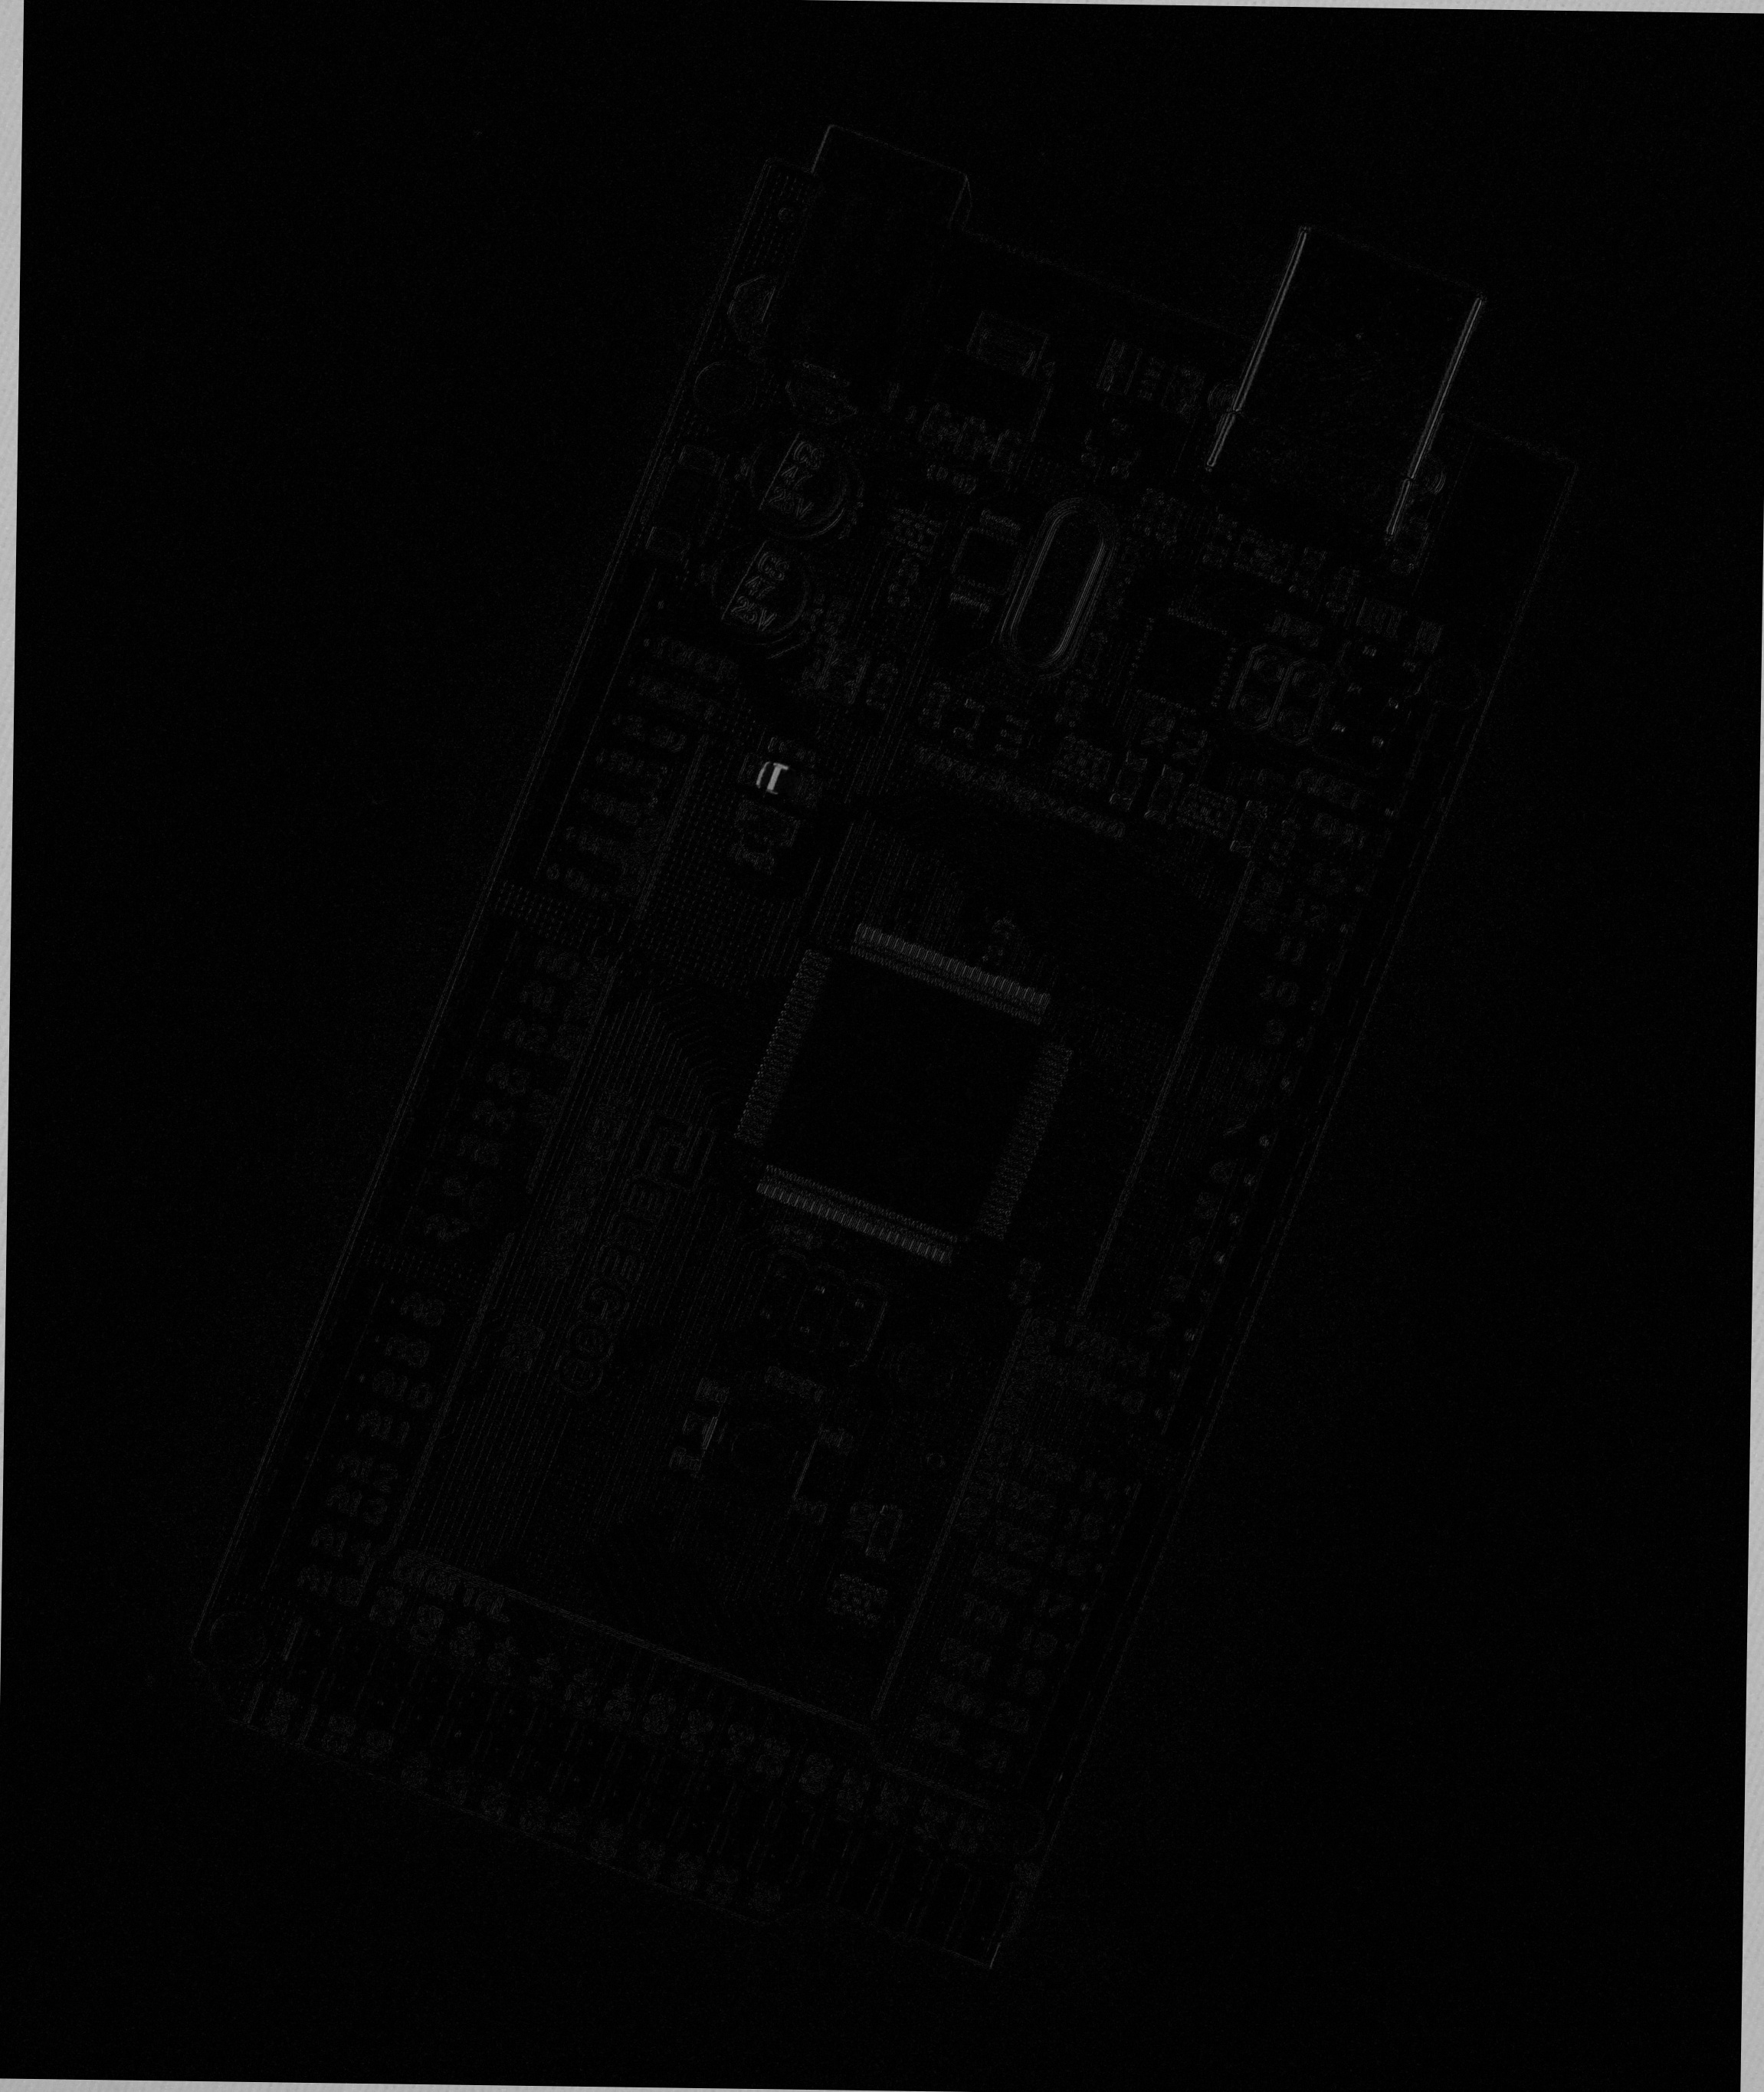
\includegraphics[width=\linewidth]{../a02 codes/diff_AECC4.jpg}
		\end{minipage}
		\vspace{-0.2cm}
		\caption{Computed difference images (\texttt{AAAA1}, \texttt{ADAD1}, \texttt{AECC2}, \texttt{AECC3}, \texttt{AECC4}). The first two show 3D parallax and lighting variations, while the last three show near-zero background residual under matched illumination.}
	\end{figure}
\end{document}